\documentclass[12pt]{article}

% ------------------------------------------------------------
% Packages
% ------------------------------------------------------------
\usepackage[a4paper,width=160mm,top=35mm,bottom=30mm,bindingoffset=0mm]{geometry}
\usepackage[T1]{fontenc}
\usepackage[utf8]{inputenc}
\usepackage{lmodern}
\usepackage{microtype}
\usepackage{graphicx}
\usepackage{xcolor}
\usepackage{float}
\usepackage{caption}
\usepackage{subcaption}
\usepackage{booktabs}
\usepackage{array}
\usepackage{tabularx}
\usepackage{longtable}
\usepackage{amsmath}
\usepackage{siunitx}
\usepackage[round,comma]{natbib}
\usepackage{ragged2e}
\usepackage{fancyhdr}
\usepackage{pdfpages}
\usepackage{tikz}
\usetikzlibrary{calc}
\usepackage{hyperref}

% ------------------------------------------------------------
% Thesis metadata
% ------------------------------------------------------------
\newcommand{\thesistitle}{Expression-Guided Comparative Evolutionary Analysis of Small Leucine-Rich Proteoglycans in Growth Plate Cartilage}
\newcommand{\thesisauthor}{Emil Vik}
\newcommand{\thesissupervisor}{Dr. Ivan Koludarov and Prof. Dr. Burkhard Rost}
% Leave empty when the two names above should remain together on one supervisor line.
% Otherwise, move the advisor's name here and remove it from \thesissupervisor.
\newcommand{\thesisadvisor}{}
\newcommand{\thesisdate}{\today}
\newcommand{\universityfrontpage}{frontmatter/university_frontpage_template.pdf}

% The supplied university PDF is a non-fillable template. These two overlays
% cover only its placeholder fields; the official LMU/TUM artwork remains intact.
\newcommand{\frontcoveroverlay}{%
  \begin{tikzpicture}[remember picture,overlay]
    \fill[white]
      ($(current page.south west)+(65pt,225pt)$)
      rectangle
      ($(current page.south west)+(530pt,390pt)$);
    \draw[line width=0.8pt]
      ($(current page.south west)+(70pt,380pt)$) --
      ($(current page.south west)+(525pt,380pt)$);
    \draw[line width=0.8pt]
      ($(current page.south west)+(70pt,290pt)$) --
      ($(current page.south west)+(525pt,290pt)$);
    \node[align=center,text width=445pt,inner sep=0pt]
      at ($(current page.south west)+(297.5pt,335pt)$)
      {\fontsize{16}{19}\selectfont\bfseries \thesistitle};
    \node[align=center,text width=445pt,inner sep=0pt]
      at ($(current page.south west)+(297.5pt,250pt)$)
      {\fontsize{12}{15}\selectfont \thesisauthor};
  \end{tikzpicture}%
}

\newcommand{\thesisadvisorrow}{}
\ifx\thesisadvisor\empty
\else
  \renewcommand{\thesisadvisorrow}{Advisor: & \thesisadvisor\\[3pt]}
\fi

\newcommand{\innertitleoverlay}{%
  \begin{tikzpicture}[remember picture,overlay]
    \fill[white]
      ($(current page.south west)+(55pt,360pt)$)
      rectangle
      ($(current page.south west)+(540pt,435pt)$);
    \node[align=center,text width=455pt,inner sep=0pt]
      at ($(current page.south west)+(297.5pt,400pt)$)
      {\fontsize{15}{18}\selectfont\bfseries \thesistitle};

    \fill[white]
      ($(current page.south west)+(55pt,85pt)$)
      rectangle
      ($(current page.south west)+(545pt,225pt)$);
    \node[anchor=north west,inner sep=0pt]
      at ($(current page.south west)+(76pt,215pt)$)
      {\begin{minipage}{455pt}
        \fontsize{11}{15}\selectfont
        \setlength{\tabcolsep}{0pt}
        \begin{tabularx}{\linewidth}{@{}>{\raggedleft\arraybackslash}p{78pt}@{\hspace{12pt}}X@{}}
          Author: & \thesisauthor\\[3pt]
          Supervisor: & \thesissupervisor\\[3pt]
          \thesisadvisorrow
          Submitted: & \thesisdate
        \end{tabularx}
      \end{minipage}};
  \end{tikzpicture}%
}

% ------------------------------------------------------------
% Hyperlinks and captions
% ------------------------------------------------------------
\hypersetup{
  colorlinks=true,
  linkcolor=black,
  urlcolor=black,
  citecolor=black
}
\captionsetup{font=footnotesize}

% ------------------------------------------------------------
% Header/footer
% ------------------------------------------------------------
\newcommand{\changefont}{\fontsize{8}{11}\selectfont}
\pagestyle{fancy}
\fancyhead{}
\fancyhead[R]{\changefont{\thesistitle}}
\fancyfoot{}
\fancyfoot[R]{\thepage}
\setlength{\headheight}{14.5pt}
\setlength{\parindent}{0pt}
\setlength{\parskip}{0.7em}
\interfootnotelinepenalty=10000

% ------------------------------------------------------------
% Document
% ------------------------------------------------------------
\begin{document}

% ------------------------------------------------------------
% Official front pages
% ------------------------------------------------------------
% The official two-page PDF is used as the background. The metadata declared
% above is placed over the template's placeholder text at compile time.
% If the PDF is missing, the fallback title page keeps the project compilable.
\IfFileExists{\universityfrontpage}{
    \includepdf[
      pages=1,
      fitpaper=true,
      pagecommand={\thispagestyle{empty}\frontcoveroverlay}
    ]{\universityfrontpage}
    \includepdf[
      pages=2,
      fitpaper=true,
      pagecommand={\thispagestyle{empty}\innertitleoverlay}
    ]{\universityfrontpage}
}{
    \begin{titlepage}
    \begin{center}
    \vspace*{2cm}
    {\Large Bioinformatics Program\\Technical University of Munich\\Ludwig-Maximilians-Universit\"at M\"unchen\par}
    \vspace{2cm}
    {\Large Bachelor Thesis in Bioinformatics\par}
    \vspace{1.5cm}
    \rule{\textwidth}{1.2pt}\\[0.4cm]
    {\LARGE\textbf{\thesistitle}\par}
    \rule{\textwidth}{1.2pt}
    \vfill
    {\Large \thesisauthor\par}
    \vspace{1cm}
    {\large Supervised by \thesissupervisor\par}
    \vspace{1cm}
    {\large Munich, \thesisdate\par}
    \end{center}
    \end{titlepage}
}

% ------------------------------------------------------------
% Front matter
% ------------------------------------------------------------
\pagenumbering{Roman}
\setcounter{page}{1}

\begin{abstract}
Small leucine-rich proteoglycans (SLRPs) organize extracellular matrix and
modulate signalling in cartilage and bone, but individual family members differ
in their direct growth-plate evidence and evolutionary assignment. This thesis
used juvenile mouse and microdissected mouse/rat growth-plate expression to
prioritize BGN, DCN, FMOD, PRELP, EPYC, LUM, and OGN, then evaluated their conservation
across representative vertebrates. Reciprocal protein searches, Pfam/HMMER,
SignalP, multiple-sequence alignment, maximum-likelihood phylogeny, protein
embeddings, representative coding-gene structure, and SynVoy microsynteny were
integrated with manual sequence review and a prioritized locus-review framework.
The curated panel contained 103 proteins, of which 102 met the current
SLRP/LRR-family criterion. SignalP calls were available for all 103 proteins:
100 were positive and three were negative. Five
genes formed pure gene-specific unrooted splits; the main LUM split contained
15 of 16 proteins, while a focused class-I diagnostic supported local BGN/DCN
discrimination despite a non-monophyletic BGN pattern. Coding-exon counts were stable
within each gene across five reference species, whereas intron-dependent locus
span varied more strongly. Comparative analysis also resolved an ASPN-like
chicken BGN-locus product, excluded an uncertain amphioxus OGN candidate, and
retained spotted-gar OGN, whale-shark EPYC, and lamprey LUM with explicit
caveats. Supplementary protein motifs supported all curated assignments, while
promoter analysis found no corrected shared targeted regulatory signature.
Together, the results support strong evolutionary constraint on a secreted
LRR-rich vertebrate ECM toolkit while demonstrating that expression,
conservation, and growth-plate function must be interpreted as distinct evidence
layers.
\end{abstract}

\newpage
\tableofcontents
\newpage
\listoffigures
\newpage
% Optional later:
% \listoftables
% \newpage

% ------------------------------------------------------------
% Main text
% ------------------------------------------------------------
\pagenumbering{arabic}
\setcounter{page}{1}

\section{Introduction}
\label{sec:introduction}
% ============================================================
% Introduction
% ============================================================
\subsection{Cartilage, the growth plate, and the extracellular matrix}
\label{subsec:cartilage-growth-plate-ecm}

Longitudinal bone growth in vertebrates occurs through endochondral ossification, a process in which a cartilage template is progressively expanded, remodeled, and replaced by bone. The growth plate is therefore not only a cellular differentiation system, but also an extracellular matrix-rich tissue whose mechanical and signalling properties depend on the composition of its matrix.
Cartilage extracellular matrix is dominated by fibrillar collagens, especially collagen type II, and by proteoglycans that contribute to hydration, tissue resilience, and the spatial organization of matrix components.

\subsection{Growth-plate zonation and a core non-SLRP gene network}
\label{subsec:growth-plate-nonslrp-network}

The epiphyseal growth plate is organized into resting, proliferative,
prehypertrophic, and hypertrophic chondrocyte compartments. These zones are
not separate tissues, but successive cellular states whose coordinated
proliferation, differentiation, matrix production, and matrix removal produce
longitudinal growth. Several non-SLRP genes provide the regulatory and matrix
framework within which the SLRPs investigated in this thesis act
(Table~\ref{tab:growth-plate-nonslrp}).

\begin{table}[H]
\centering
\caption{Representative non-SLRP genes in growth-plate organization. The
selection summarizes major regulatory and matrix modules and is not intended
as an exhaustive catalogue of all genes expressed in growth-plate cartilage.}
\label{tab:growth-plate-nonslrp}
\begin{tabularx}{\textwidth}{@{}p{0.27\textwidth}X@{}}
\toprule
Gene or pathway & Principal growth-plate role \\
\midrule
\textit{SOX9}, \textit{COL2A1}, and \textit{ACAN} &
SOX9 is essential for chondrocyte lineage formation and supports expression of
cartilage-matrix genes including type-II collagen and aggrecan. These matrix
components provide the collagenous and hydrated proteoglycan framework in
which SLRPs are embedded \citep{Bi1999Sox9}. \\
\textit{IHH}, \textit{PTHLH}, and \textit{PTH1R} &
The IHH--PTHrP feedback system couples the position of prehypertrophic cells to
the rate at which proliferating chondrocytes enter hypertrophy, thereby
preventing premature terminal differentiation \citep{Vortkamp1996IhhPthrp}. \\
\textit{RUNX2} and \textit{COL10A1} &
RUNX2 is required for normal chondrocyte proliferation and maturation during
endochondral ossification. Type-X collagen is a characteristic component of
hypertrophic cartilage and marks the matrix state that precedes replacement by
bone \citep{Chen2014Runx2}. \\
\textit{FGFR3} &
FGFR3 limits endochondral bone growth; disruption of the receptor in mice
expands proliferating and hypertrophic growth-plate compartments, whereas
activating human variants cause skeletal dysplasias such as achondroplasia
\citep{Deng1996Fgfr3}. \\
\textit{NPPC} and \textit{NPR2} &
Locally produced C-type natriuretic peptide signals through NPR2/guanylyl
cyclase-B and positively supports endochondral ossification and longitudinal
bone growth \citep{Tamura2004Npr2}. \\
\textit{MMP13} &
MMP13 cleaves cartilage matrix during the hypertrophic-to-ossification
transition. Loss of MMP13 causes collagen accumulation, enlargement of the
hypertrophic zone, and delayed ossification and vascularization
\citep{Inada2004Mmp13}. \\
\textit{VEGFA} &
VEGF produced by hypertrophic chondrocytes promotes vascular invasion and
couples terminal cartilage remodeling to trabecular bone formation
\citep{Gerber1999Vegf}. \\
\bottomrule
\end{tabularx}
\end{table}

This framework separates different kinds of evidence. SOX9, IHH--PTHrP,
RUNX2, FGFR3, and CNP--NPR2 primarily regulate chondrocyte state or growth;
COL2A1, ACAN, and COL10A1 define changing matrix environments; and MMP13 and
VEGFA help execute the cartilage-to-bone transition. The focal SLRPs are best
placed within the matrix branch of this system: their conserved secretion
signals, leucine-rich repeat architecture, and collagen-associated functions
make them plausible modifiers of the extracellular environment, but do not by
themselves establish that an SLRP controls growth-plate zonation. These
non-SLRP genes therefore provide biological context rather than an additional
comparative candidate set in the present study.

\subsection{Proteoglycans and small leucine-rich proteoglycans}
\label{subsec:proteoglycans-slrps}

Small leucine-rich proteoglycans (SLRPs) are extracellular matrix proteins characterized by a relatively small core protein and a central leucine-rich repeat domain. This domain forms a curved interaction surface that enables binding to collagens, growth factors, and other matrix-associated molecules. Although historically described mainly as structural matrix components, SLRPs are now understood as multifunctional regulators of matrix assembly, tissue mechanics, mineralization, and cell signalling \citep{SchaeferIozzo2008,IozzoSchaefer2015}.

\subsection{SLRPs in collagen-rich skeletal tissues}
\label{subsec:slrps-skeletal-tissues}

SLRPs influence collagen-rich tissues by binding to fibrillar collagens and modulating fibril assembly, spacing, and susceptibility to proteolytic degradation. This is particularly relevant in cartilage, where matrix remodeling accompanies both normal skeletal development and pathological degeneration. For example, fibromodulin is processed by cartilage-associated proteases such as MMP-13 and ADAMTS enzymes, and MMP-13-cleaved fibromodulin has been detected in hypertrophic chondrocytes of human fetal growth plates.

\subsection{Evolutionary origin and species sampling}
\label{subsec:slrp-evolutionary-origin}

Comparative studies indicate that an ancestral SLRP-like protein was probably
present early in chordate evolution and that the family expanded during early
vertebrate evolution. Tunicates such as \textit{Ciona} contain a small number
of SLRP-like genes that have been discussed as possible precursors of the
canonical vertebrate family, whereas early-diverging vertebrates already show
several distinguishable SLRP-like genes \citep{Park2008}. A broadly recognizable
modern repertoire was established before the divergence of cartilaginous and
bony vertebrates, followed by lineage-specific changes including teleost gene
duplication \citep{Costa2018}. A more recent comparative survey describes
both whole-genome and tandem duplication as contributors to the expansion of
clustered SLRP genes in jawed vertebrates \citep{Gil2025}.

No living species is treated here as the ancestor from which the other sampled
species evolved. Instead, amphioxus, lamprey, cartilaginous fishes, spotted gar,
coelacanth, teleosts, and tetrapods bracket informative stages of chordate and
vertebrate history. \textit{Ciona} is retained as literature-only family-origin
context because its SLRP-like sequence cannot be assigned confidently to BGN,
DCN, FMOD, PRELP, EPYC, LUM, or OGN. Amphioxus defines a deep chordate
uncertainty boundary; lamprey tests early vertebrate diversification; sharks
represent the earliest sampled jawed-vertebrate branch; and gar and coelacanth
help distinguish ancient vertebrate conservation from teleost-specific
duplication.

\subsection{Candidate genes investigated in this thesis}
\label{subsec:candidate-genes}

The comparative panel comprises \textit{BGN}, \textit{DCN}, \textit{FMOD},
\textit{PRELP}, \textit{EPYC}, \textit{LUM}, and \textit{OGN}. These genes were not selected
because RNA abundance alone demonstrates function. They represent several SLRP
classes and combine juvenile-lineage expression with different degrees of
growth-plate localization, skeletal function, and collagen-matrix evidence.
The literature also makes clear that SLRPs are partly redundant: a mild
single-gene phenotype can coexist with a stronger compound-knockout phenotype,
whereas a compound knockout cannot identify the separate contribution of each
protein \citep{Nikitovic2012}.

\subsubsection{Biglycan, decorin, and fibromodulin}

\textit{BGN} encodes biglycan, a class-I chondroitin/dermatan-sulphate SLRP
abundant in skeletal connective tissues. Biglycan contributes to collagen-fibril
organization, osteogenesis, and bone remodelling. Biglycan-deficient mice show
abnormal collagen fibrils and reduced skeletal growth or bone mass, with a much
stronger phenotype after combined loss of the related class-I SLRP decorin
\citep{Corsi2002}. Biglycan therefore has both a structural matrix role and
context-dependent effects on bone-cell signalling; the relative contribution of
these mechanisms within individual growth-plate zones remains unresolved.

\textit{DCN} encodes decorin, a closely related class-I SLRP with established
roles in collagen fibrillogenesis, cartilage matrix organization, and cell-
matrix signalling. It was included both as a biologically relevant candidate
and as the essential paralog control for testing whether apparent BGN sequences
were actually decorin-like records.

\textit{FMOD} encodes fibromodulin, a class-II collagen-binding SLRP. Loss of
fibromodulin disrupts tendon collagen-fibril morphology and alters lumican
deposition, demonstrating an in-vivo role in collagen fibrillogenesis and
partial functional overlap with other SLRPs \citep{Svensson1999}. During mouse
knee development, fibromodulin is enriched in growing epiphyses and localizes
around late-hypertrophic chondrocytes, the secondary ossification centre, and
the growth plate \citep{Saamanen2001}. FMOD is also cleaved by cartilage-
remodelling proteases, and MMP-13-cleaved fibromodulin occurs around
hypertrophic chondrocytes in fetal growth plates \citep{Shu2019}.

BGN and FMOD also influence skeletal remodelling together. Their combined loss
in mice increases osteoclastogenesis and produces low bone mass, while both
proteins can interact with TNF-alpha and RANKL in experimental systems
\citep{Kram2017}. However, incomplete rescue of the double-knockout phenotype by
OPG-Fc, together with adverse effects in young mice, shows that this biology
cannot be reduced to a single osteoclast pathway \citep{Kram2020}.

\subsubsection{PRELP}

\textit{PRELP} encodes a class-II extracellular LRR protein distinguished by a
basic proline/arginine-rich N-terminus. This N-terminal region binds heparin and
heparan sulphate and may link matrix components to cell-surface heparan-sulphate
proteoglycans \citep{Bengtsson2000}. PRELP is present in cartilage, and its LRR,
cysteine, and glycosylation-associated regions are conserved between human and
mouse \citep{Grover1996,Grover2002}. PRELP-derived N-terminal peptides inhibit
osteoclast differentiation and can reduce bone loss in experimental models,
whereas cell-culture work also supports a role in osteoblast differentiation
\citep{Rucci2009,Rucci2013,Li2016PRELP}. Peptide pharmacology and cultured-cell
effects do not yet establish the normal function of endogenous full-length PRELP
in the growth plate, so its precise in-vivo mechanism remains incomplete.

\subsubsection{Epiphycan}

\textit{EPYC} encodes epiphycan/PG-Lb, a class-III cartilage-enriched
chondroitin/dermatan-sulphate SLRP. In embryonic mouse limbs, \textit{Epyc} RNA
is associated mainly with resting and proliferating chondrocytes, while the
secreted protein is distributed throughout the growth-plate matrix, including
around hypertrophic chondrocytes \citep{Johnson1999}. Epyc-null mice are viable
and lack a severe early skeletal phenotype, but develop age-related joint and
femur-length abnormalities; earlier or stronger osteoarthritis in
Epyc/Bgn-deficient mice indicates interaction and compensation between SLRPs
\citep{Nuka2010}. EPYC therefore has direct anatomical relevance to the growth
plate, but its specific molecular binding partners and indispensable mechanism
remain less well defined than its distribution.

\subsubsection{Lumican}

\textit{LUM} encodes lumican, a widely distributed class-II collagen-binding
SLRP. Lumican regulates collagen-fibril diameter and organization in several
connective tissues and has partly overlapping functions with fibromodulin.
During skeletal development it is present in cartilaginous and developing bone
matrices \citep{Raouf2002}. Lumican knockdown in tissue-engineered cartilage
increased type-II collagen deposition and fibril diameter, demonstrating that
its effect on collagen accumulation is context dependent rather than simply
``pro-collagen'' \citep{Kafienah2008}. Recombinant lumican also suppresses
osteoclast differentiation and resorption through reduced Akt activity in
vitro \citep{Lee2021Lum}; whether this mechanism operates at physiologically
important levels in the juvenile growth plate remains unknown.

\subsubsection{Osteoglycin}

\textit{OGN}, also known as mimecan, encodes a class-III secreted SLRP. Ogn-null
mice are viable without an obvious gross developmental phenotype, but show
abnormal collagen fibril diameter and morphology in skin and cornea, providing
in-vivo evidence for collagen-fibrillogenesis control \citep{Tasheva2002}.
BMP1/Tolloid-family metalloproteinases process pro-OGN and enhance its regulation
of type-I collagen fibrillogenesis in biochemical assays \citep{Ge2004}.
Vertebrate OGN history also includes teleost duplication and
subfunctionalization \citep{Costa2018}. OGN therefore contributes an informative
evolutionary and matrix-remodelling case, but it has weaker direct evidence for
a growth-plate-specific function than FMOD or EPYC.

\subsubsection{Osteomodulin as a context gene}

\textit{OMD}/osteoadherin is not a seventh fully analysed panel member, but it
provides relevant cartilage--bone-interface context. The secreted protein binds
hydroxyapatite, supports integrin-associated osteoblast attachment, and is
localized to the primary spongiosa of fetal growth plates \citep{Sommarin1998}.
OMD has also been linked to BMP2/SMAD-dependent osteogenesis
\citep{Lin2021OMD}. Its expression and representative gene structure are
reported here, but it did not undergo the complete protein, phylogenetic, and
synteny workflow.

Together, these studies justify the panel as a set of biologically plausible
cartilage and skeletal ECM genes while also defining the limits of the thesis.
The comparative analyses can test ortholog plausibility and conservation of
secretion, LRR architecture, sequence, gene structure, phylogenetic placement,
and genomic neighbourhood. They cannot demonstrate that every ortholog has the
same collagen-binding, signalling, or growth-plate phenotype.

\subsection{Expression-guided evolutionary analysis}
\label{subsec:expression-guided-evolution}

Because SLRPs form a multi-gene family with related domain architectures and partially overlapping functions, sequence similarity alone may not be sufficient to distinguish orthologs from closely related paralogs. Combining expression evidence with reciprocal sequence searches, domain validation, phylogenetic reconstruction, and synteny analysis can therefore provide a more reliable framework for identifying conserved cartilage-associated SLRP candidates across vertebrates.

\subsection{Aim of this thesis}
\label{subsec:aim}

This thesis aims to characterize selected growth-plate-associated SLRP genes by
combining juvenile and anatomically resolved expression evidence with
comparative analyses across representative vertebrates. Specifically, it asks
which SLRPs form a biologically justified candidate panel, whether their
secretory signals, LRR-rich protein cores, coding organization, phylogenetic
identity, and genomic neighbourhoods are conserved, and where deep-lineage or
annotation uncertainty limits an ortholog assignment. By integrating these
independent evidence layers, the work distinguishes a conserved vertebrate ECM
framework from candidate-specific expression differences, paralogy, and gene-
model uncertainty.


\newpage
\section{Results}
\label{sec:results}
% ============================================================
% Results draft generated from the frozen analysis tables.
% Replace cross-references after final figure/table numbering is fixed.
% ============================================================

\subsection{Expression-guided selection of candidate SLRPs}
\label{subsec:results-expression}

The initial expression screen measured nine SLRP genes in three samples of
P0-derived Prx1-lineage chondrocyte material from NCBI GEO GSE305415. BGN had the
highest mean abundance (3012.762 TPM), followed by OGN (657.412 TPM), FMOD
(605.864 TPM), DCN (581.246 TPM), LUM (272.457 TPM), PRELP (189.840 TPM),
ASPN (112.954 TPM),
EPYC (99.059 TPM), and OMD (96.317 TPM). Because these samples represented a
P0-derived skeletal lineage rather than anatomically isolated growth-plate zones,
the screen was treated as a prioritization dataset and not as direct evidence
of growth-plate-specific expression. The deposited series and sample records
disagree about whether RNA was extracted before or after culture; therefore,
these values were not attributed to an exact in-vivo chondrocyte state.

Processed microdissected tibial growth-plate data from mouse and rat
(GSE114919) provided the direct anatomical comparison. BGN, FMOD, and PRELP
ranked consistently highly across the examined age-by-zone conditions. LUM and
EPYC showed intermediate support, whereas OGN ranked lower, particularly in
rat. The numerical scales of the GSE305415-derived TPM dataset and GSE114919
were not pooled. Bgee call summaries and gene-specific literature were used as
independent contextual evidence rather than as replacements for the two
expression analyses. Figure~\ref{fig:expression-evidence} presents these two
complementary expression layers without combining their numerical scales.

The final comparative panel therefore comprised BGN, DCN, FMOD, PRELP, EPYC,
LUM, and OGN. Selection was not based on abundance alone: the panel also represented
SLRP classes I--III, included genes with direct cartilage or skeletal evidence,
and retained OGN as an explicitly exploratory class-III member. DCN was included
as a full class-I candidate and the closest paralog control for BGN. OMD was
retained as a context gene because of its
skeletal literature and conserved representative gene structure, but it was not
advanced to the full protein, phylogeny, and synteny workflow. ASPN was retained
as class-I background rather than advanced to the seven-gene panel: it ranked
seventh in the P0-derived screen, its independent tibial growth-plate support
was weaker and inconsistent between mouse and rat, and BGN plus the DCN paralog
control already supplied the main class-I comparison. This was a scope and
evidence-prioritization decision, not a claim that ASPN is absent from cartilage.

\begin{figure}[htbp]
    \centering
    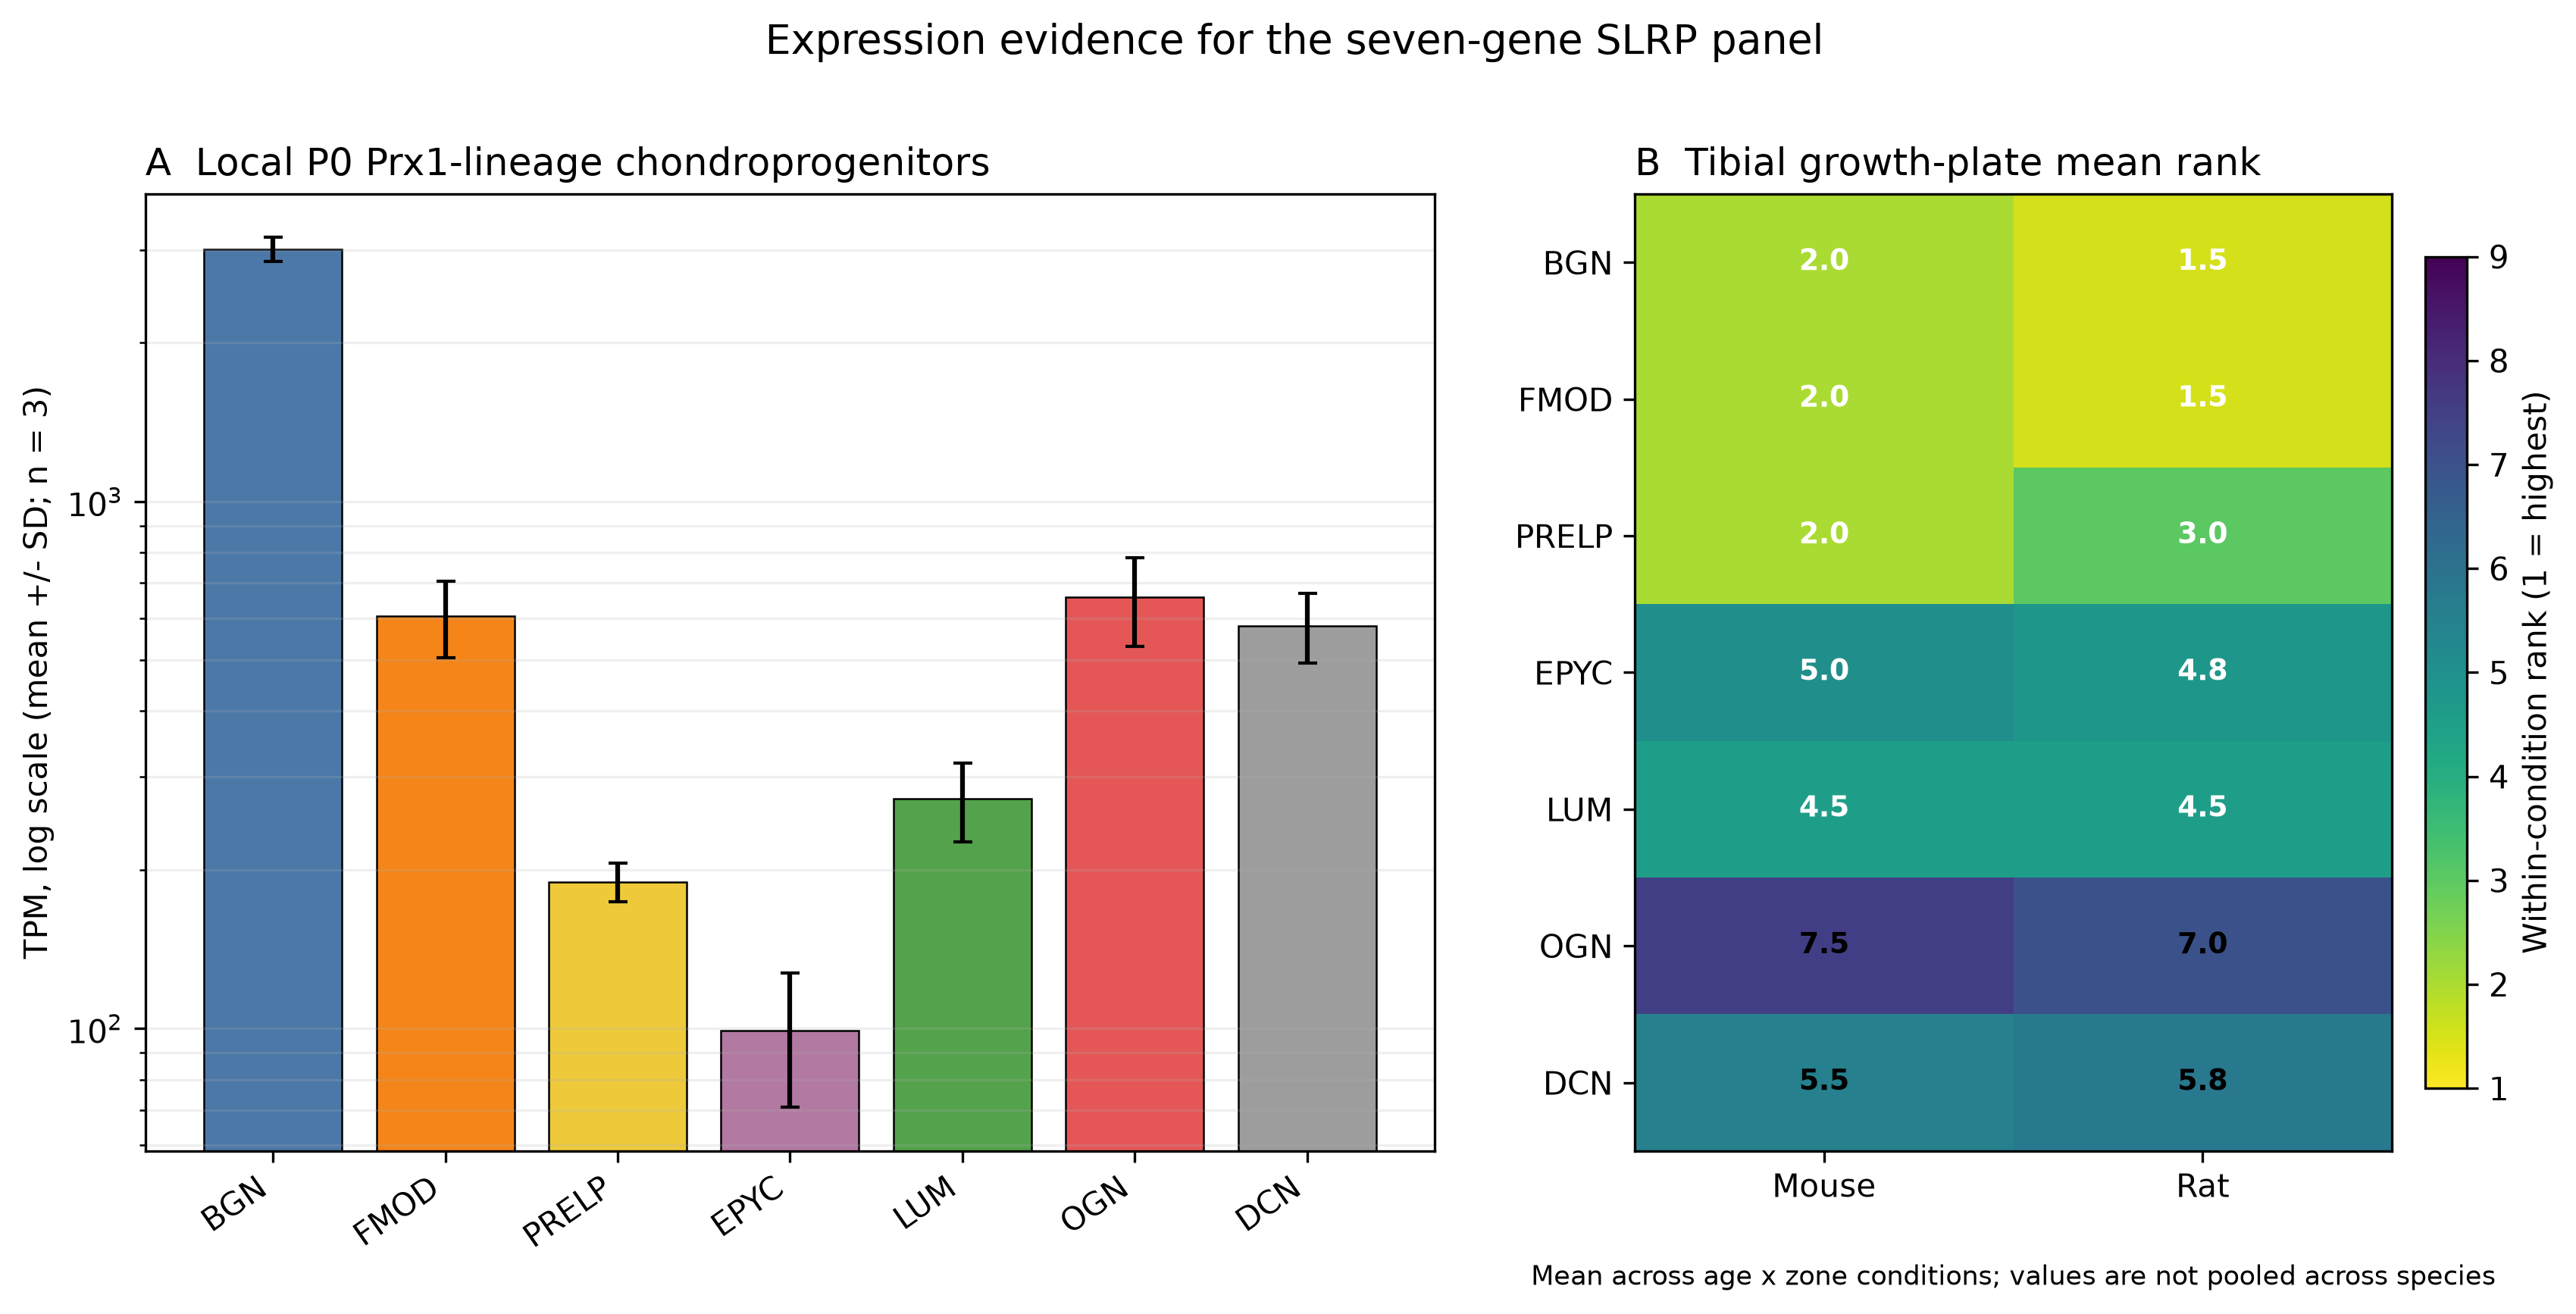
\includegraphics[width=\textwidth,height=0.76\textheight,keepaspectratio]
        {figures/expression/expression_evidence.png}
    \caption{Expression evidence used to prioritize the seven-gene SLRP panel.
    Panel A summarizes mean expression in three samples of P0-derived
    Prx1-lineage chondrocyte material from NCBI GEO GSE305415; error bars show
    standard deviation and the abundance axis is logarithmic. Panel B
    summarizes within-condition ranks in
    processed mouse and rat microdissected tibial growth-plate data
    (GSE114919). The two numerical scales were not pooled. Expression was used
    for biological prioritization and does not establish function or orthology.
    Because the deposited records conflict about culture before RNA extraction,
    the exact cell state is not assigned.}
    \label{fig:expression-evidence}
\end{figure}

\subsection{Cross-species candidate recovery and manual protein curation}
\label{subsec:results-protein-conservation}

After reciprocal-hit, annotation, length, and duplication checks, the confident
canonical panel contained 103 nonredundant proteins: BGN 13, DCN 15, FMOD 14,
PRELP 16, EPYC 15, LUM 16, and OGN 14. Four historical BGN assignments were
removed as DCN or DCN-like records, and tentative partial replacement models
were retained for catshark and whale shark. The amphioxus sequence
\texttt{XP\_066265713.1} was removed from the confident OGN ortholog set after
manual alignment review and disagreement among tree, synteny, and reciprocal-hit
evidence. It was retained only as an uncertain SLRP-like provenance record. The
chicken BGN-locus product \texttt{XP\_414298.2} was likewise excluded from the
canonical BGN protein set because its product annotation, reciprocal hit, and a
focused reference tree supported ASPN rather than BGN.

\subsubsection{Conserved domain architecture and alignment continuity}

Across the final panel, 102 of 103 proteins met the current SLRP/LRR-family
criterion. SignalP results were available for all 103 proteins: 100 were
positive and three were negative. The final 17-sequence run produced 15
positive calls; its negative calls were the fragmentary whale-shark BGN
\texttt{XP\_048475905.1} and opossum DCN \texttt{XP\_001363160.3}. The third
negative record was spotted-gar OGN \texttt{XP\_006631165.2}. Manual inspection
showed an intact OGN protein and a continuous LRR-rich alignment, so it was
retained as tentative while uncertainty about its N-terminal secretion signal
was recorded. The exact spotted-gar GFF contained only one \textit{ogna}
transcript (\texttt{XM\_006631102.3}), so no annotated alternative N terminus
could be substituted. Although residues 8--25 form a strongly hydrophobic
N-terminal segment, SignalP classified the sequence as OTHER (SP score 0.167)
without a cleavage call; this supported no confidence upgrade. Opossum OGN
\texttt{XP\_056660002.1} and zebrafish OGN \texttt{NP\_001013588.1} were
retained after manual inspection of termini, conserved cysteine positions, and
alignment continuity. The whale-shark EPYC sequence
\texttt{XP\_048463897.1} was retained as tentative. Manual inspection found a
similar early N-terminal beginning and a strongly conserved
middle-to-C-terminal region, but numerous mismatches in the earlier portion,
reduced query coverage, and an alternative reciprocal hit prevented an
unqualified assignment.

Focused review resolved the four outstanding class-I protein questions.
Catshark BGN \texttt{XP\_038638277.1} has a strong signal peptide, conserved
comparable cysteines and SLRP/LRR domains, but lacks approximately 111
human-equivalent C-terminal residues; it was retained as a tentative partial
ortholog. Whale-shark BGN \texttt{XP\_048475905.1} is a discontinuous 161-aa
fragment at a syntenically supported BGN locus and lacks a detectable signal
peptide; it was retained only as a tentative locus/fragment record and excluded
from complete-protein claims. Opossum DCN \texttt{XP\_001363160.3} is a highly
conserved C-terminal fragment that lacks the N-terminal signal-peptide region;
its protein assignment was retained, while its locus remained unresolved
because the SynVoy FASTA and GFF versions do not match. Catshark DCN
\texttt{XP\_038636759.1} spans the full aligned core, retains all six comparable
cysteines, lies in the DCN tree split and has a SignalP-positive N terminus. It
was retained confidently, with its 29-aa N-terminal extension and predicted
cleavage between residues 45 and 46 recorded as a gene-model caveat.

All seven gene-specific alignments retained a conserved core despite variation at
the termini and in gap-rich regions. Exact amino-acid identity was not required
for orthology: manual review emphasized intact termini, conserved cysteines,
continuous alignment through the LRR-rich region, absence of large
sequence-specific insertions or deletions, and agreement with independent tree,
synteny, and SignalP evidence. Figure~\ref{fig:protein-conservation} summarizes
the alignment, domain, signal-peptide, and candidate-level quality-control
evidence across the final 103-protein panel.

\begin{figure}[htbp]
    \centering
    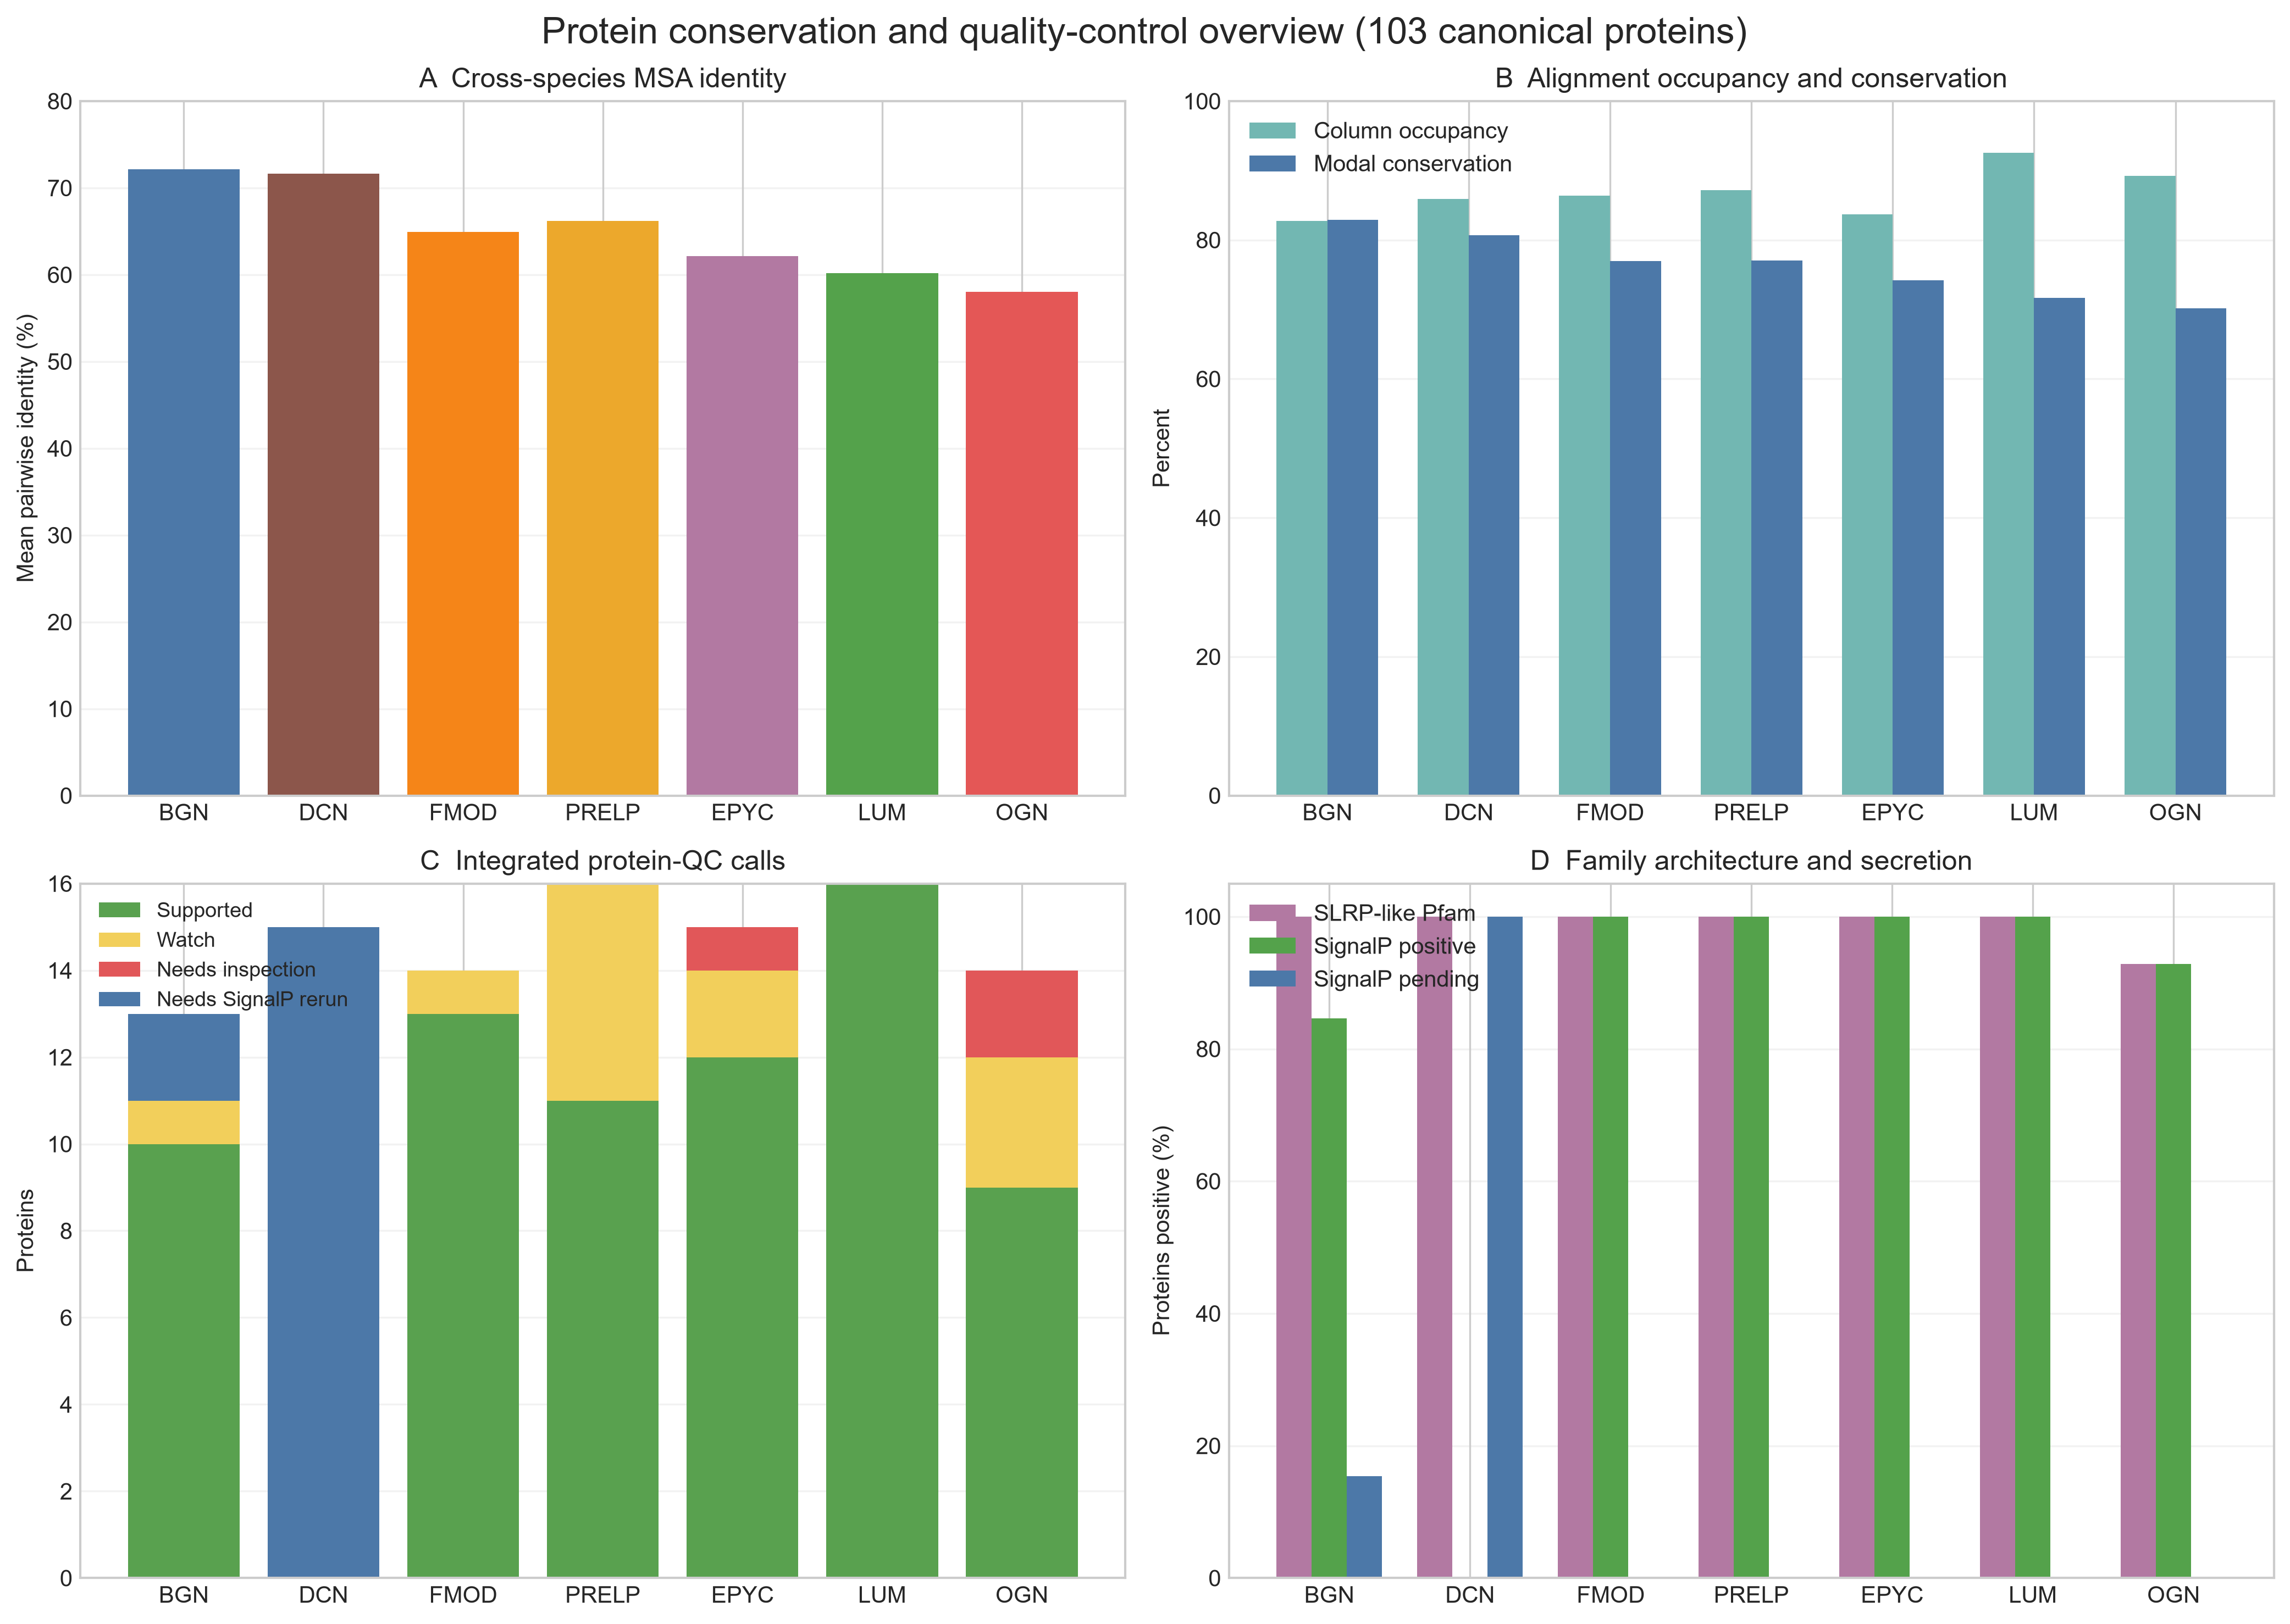
\includegraphics[width=\textwidth,height=0.76\textheight,keepaspectratio]
        {figures/protein/protein_conservation_overview.png}
    \caption{Protein conservation and quality-control summary for the
    103-protein canonical SLRP panel. The panels summarize within-gene sequence
    identity, alignment occupancy and modal-residue conservation, integrated
    candidate flags, Pfam SLRP/LRR-family support, and SignalP-positive calls.
    SignalP results are complete for all 103 proteins (100 positive and three
    negative). These measures
    support conserved secreted SLRP architecture but do not individually prove
    gene-specific orthology or conserved biological function.}
    \label{fig:protein-conservation}
\end{figure}

\subsection{Phylogenetic support for gene-specific assignments}
\label{subsec:results-phylogeny}

Maximum-likelihood trees were inferred from the curated per-gene alignments and
from a trimmed alignment of all 103 proteins. DCN, EPYC, FMOD, PRELP, and the
revised 14-sequence OGN set formed gene-specific unrooted splits in the combined
tree. The main LUM split contained 15 of 16 LUM proteins; lamprey
\texttt{XP\_075930353.1} occurred outside this split among closely related
class-II sequences. The lamprey record was retained once as a tentative
deep-lineage LUM assignment because its annotation and reciprocal evidence were
compatible with lumican, but the tree did not support an unqualified assignment.
BGN did not form one pure split after DCN was included: the largest pure BGN
split contained 6 of 13 tips. A focused class-I analysis nevertheless found a
closer BGN tip than DCN tip for every BGN sequence and the reciprocal pattern
for every DCN sequence. This supported coherent local BGN/DCN discrimination
while preserving caution about partial deep-lineage BGN models. The trees were interpreted as unrooted orthology evidence; they were not used to
infer a direction of evolution without an explicit outgroup. The combined
analysis and its gene-specific exceptions are shown in
Figure~\ref{fig:combined-phylogeny}.

\begin{table}[htbp]
    \centering
    \caption{Support for the largest pure gene-specific split in the final
    103-protein unrooted tree. Branch labels are reported as
    SH-aLRT/UFBoot percentages. For BGN and LUM the value describes the largest
    pure subset rather than monophyly of every assigned sequence.}
    \label{tab:phylogeny-support}
    \begin{tabularx}{\textwidth}{@{}lcccX@{}}
        \toprule
        Gene & Pure split & Total tips & SH-aLRT/UFBoot & Interpretation \\
        \midrule
        BGN   & 6  & 13 & 99.6/99 & Strongly supported subset; the full BGN set is not one pure split. \\
        DCN   & 15 & 15 & 100/99  & Complete pure split. \\
        EPYC  & 15 & 15 & 96.6/89 & Complete pure split. \\
        FMOD  & 14 & 14 & 94/100  & Complete pure split. \\
        OGN   & 14 & 14 & 94.9/99 & Complete pure split after amphioxus exclusion. \\
        PRELP & 16 & 16 & 94.3/99 & Complete pure split. \\
        LUM   & 15 & 16 & 94.1/99 & Main pure split; lamprey LUM lies outside it. \\
        \bottomrule
    \end{tabularx}
\end{table}

\begin{figure}[p]
    \centering
    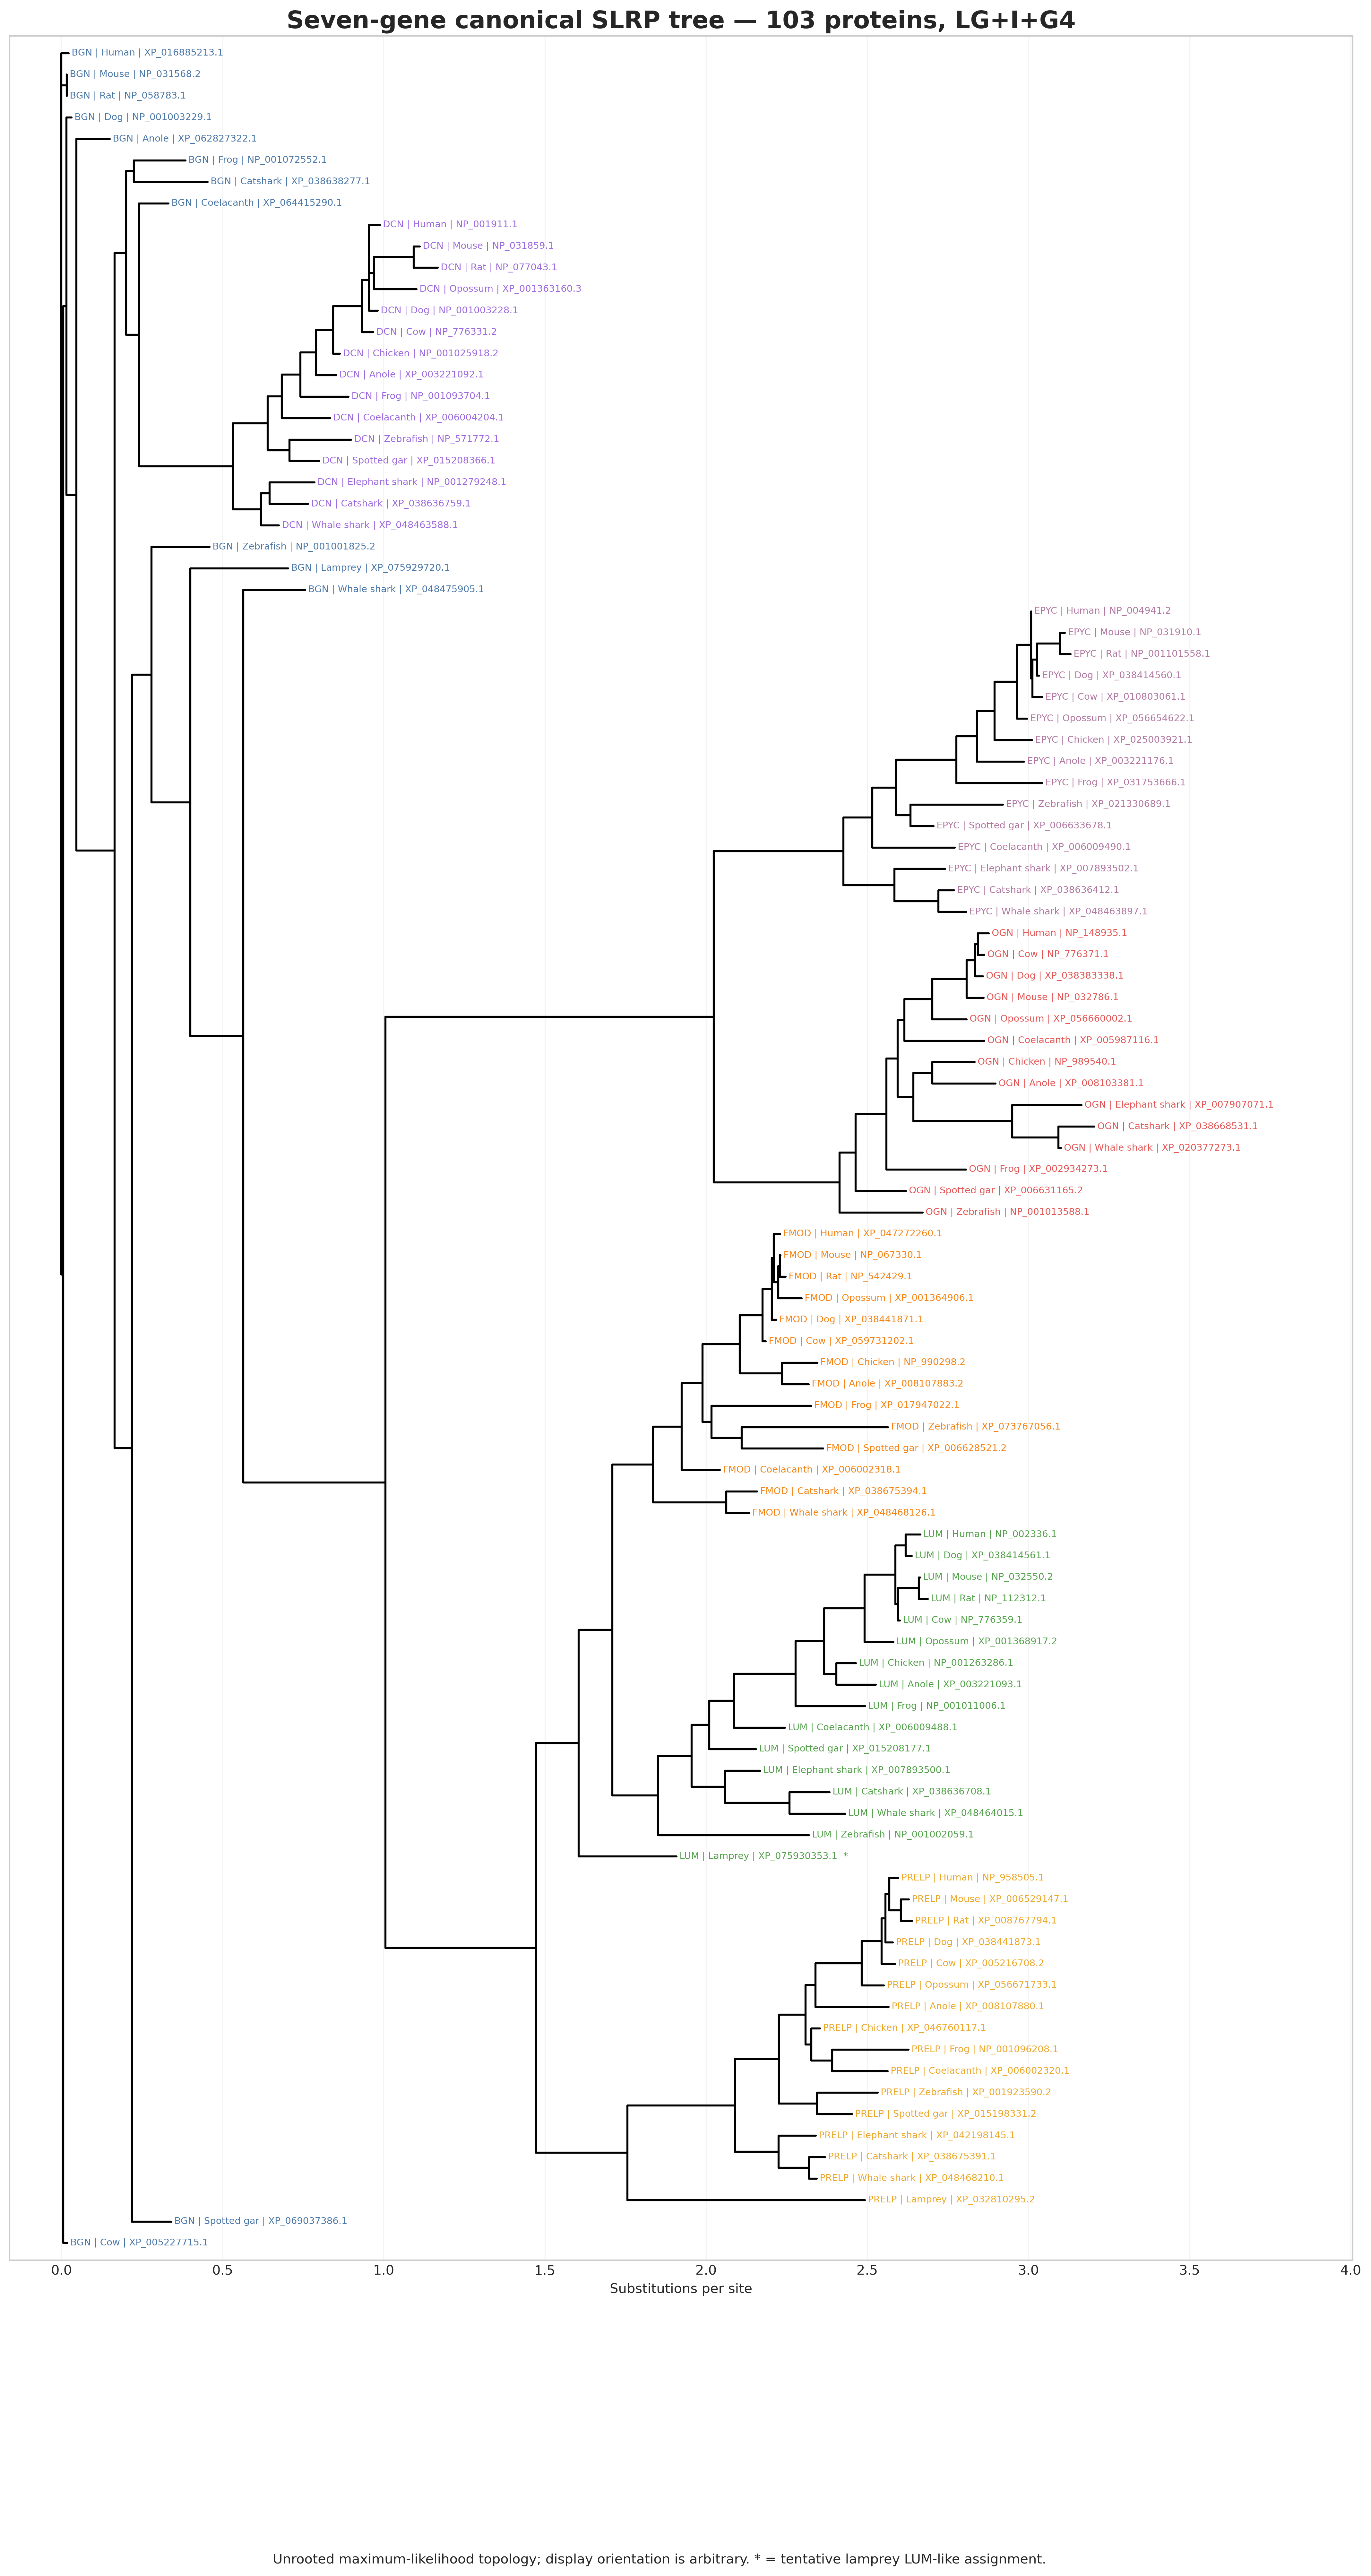
\includegraphics[width=\textwidth,height=0.82\textheight,keepaspectratio]
        {figures/phylogeny/combined_103_protein_tree.png}
    \caption{Unrooted maximum-likelihood phylogeny of the curated 103-protein
    SLRP panel. Tip colours denote the seven gene assignments. DCN, EPYC, FMOD,
    OGN, and PRELP form pure gene-specific unrooted splits; the main LUM split
    contains 15 of 16 sequences, while lamprey LUM is retained tentatively.
    BGN requires the focused BGN/DCN diagnostic rather than interpretation as a
    single pure split. Display orientation does not imply evolutionary
    direction.}
    \label{fig:combined-phylogeny}
\end{figure}

The broader NCBI search was used as a species-expansion analysis rather than as
a replacement for the curated tree. Corrected one-per-locus candidate sets
contained 639 BGN, 632 EPYC, 546 FMOD, 838 LUM, 855 OGN, and 848 PRELP records.
This shows that the workflow can recover homologous candidates far beyond the
15-species panel, but these counts are search outputs rather than verified
ortholog counts. The previously generated large trees were affected by a header-
parsing error that could collapse unrelated loci carrying the same isoform label.
Their topologies are therefore excluded from the thesis evidence. Corrected
large-tree inference remains optional because the curated 103-protein analysis
already answers the principal comparative question.

The targeted species panel provided a separate evolutionary bracket. Amphioxus
did not yield a confident OGN ortholog and instead supplied an informative
SLRP-like uncertainty case. Lamprey retained distinguishable deep-vertebrate
SLRP-like candidates, although the tentative LUM placement showed that closely
related class-II genes remain difficult to resolve at this depth. Cartilaginous-
fish candidates extended recognizable gene-specific architecture to an early
jawed-vertebrate branch but also contained the most obvious partial and
annotation-sensitive BGN/EPYC models. Spotted gar and coelacanth bridged these
deep comparisons to teleosts and tetrapods, allowing teleost divergence or
duplication to be distinguished from loss of ancient vertebrate conservation.
These living species were interpreted as comparative representatives, not as
ancestors of the other sampled lineages.

The species-level summary made this evolutionary pattern quantitative
(Figure~\ref{fig:species-lineage-summary}). Median amino-acid identity to the
human reference was lowest in the three retained lamprey proteins (48.5\%) and
the elephant-shark and catshark sets (51.2\% and 53.2\%), and increased to
85.0--93.5\% in non-human mammals. This trend was not a simple phylogenetic
ladder: spotted gar had a higher median identity (68.1\%) than zebrafish
(61.2\%) or coelacanth (59.8\%). Different gene subsets, lineage-specific rates,
and gene-model quality all contribute to these descriptive medians. Manual
synteny review accepted five of seven loci in both spotted gar and coelacanth,
compared with three of seven in each sampled shark. Amphioxus produced no
accepted gene-specific locus, whereas the seven ambiguous opossum results
reflected incompatible FASTA/GFF inputs rather than evolutionary divergence.

\begin{figure}[tbp]
    \centering
    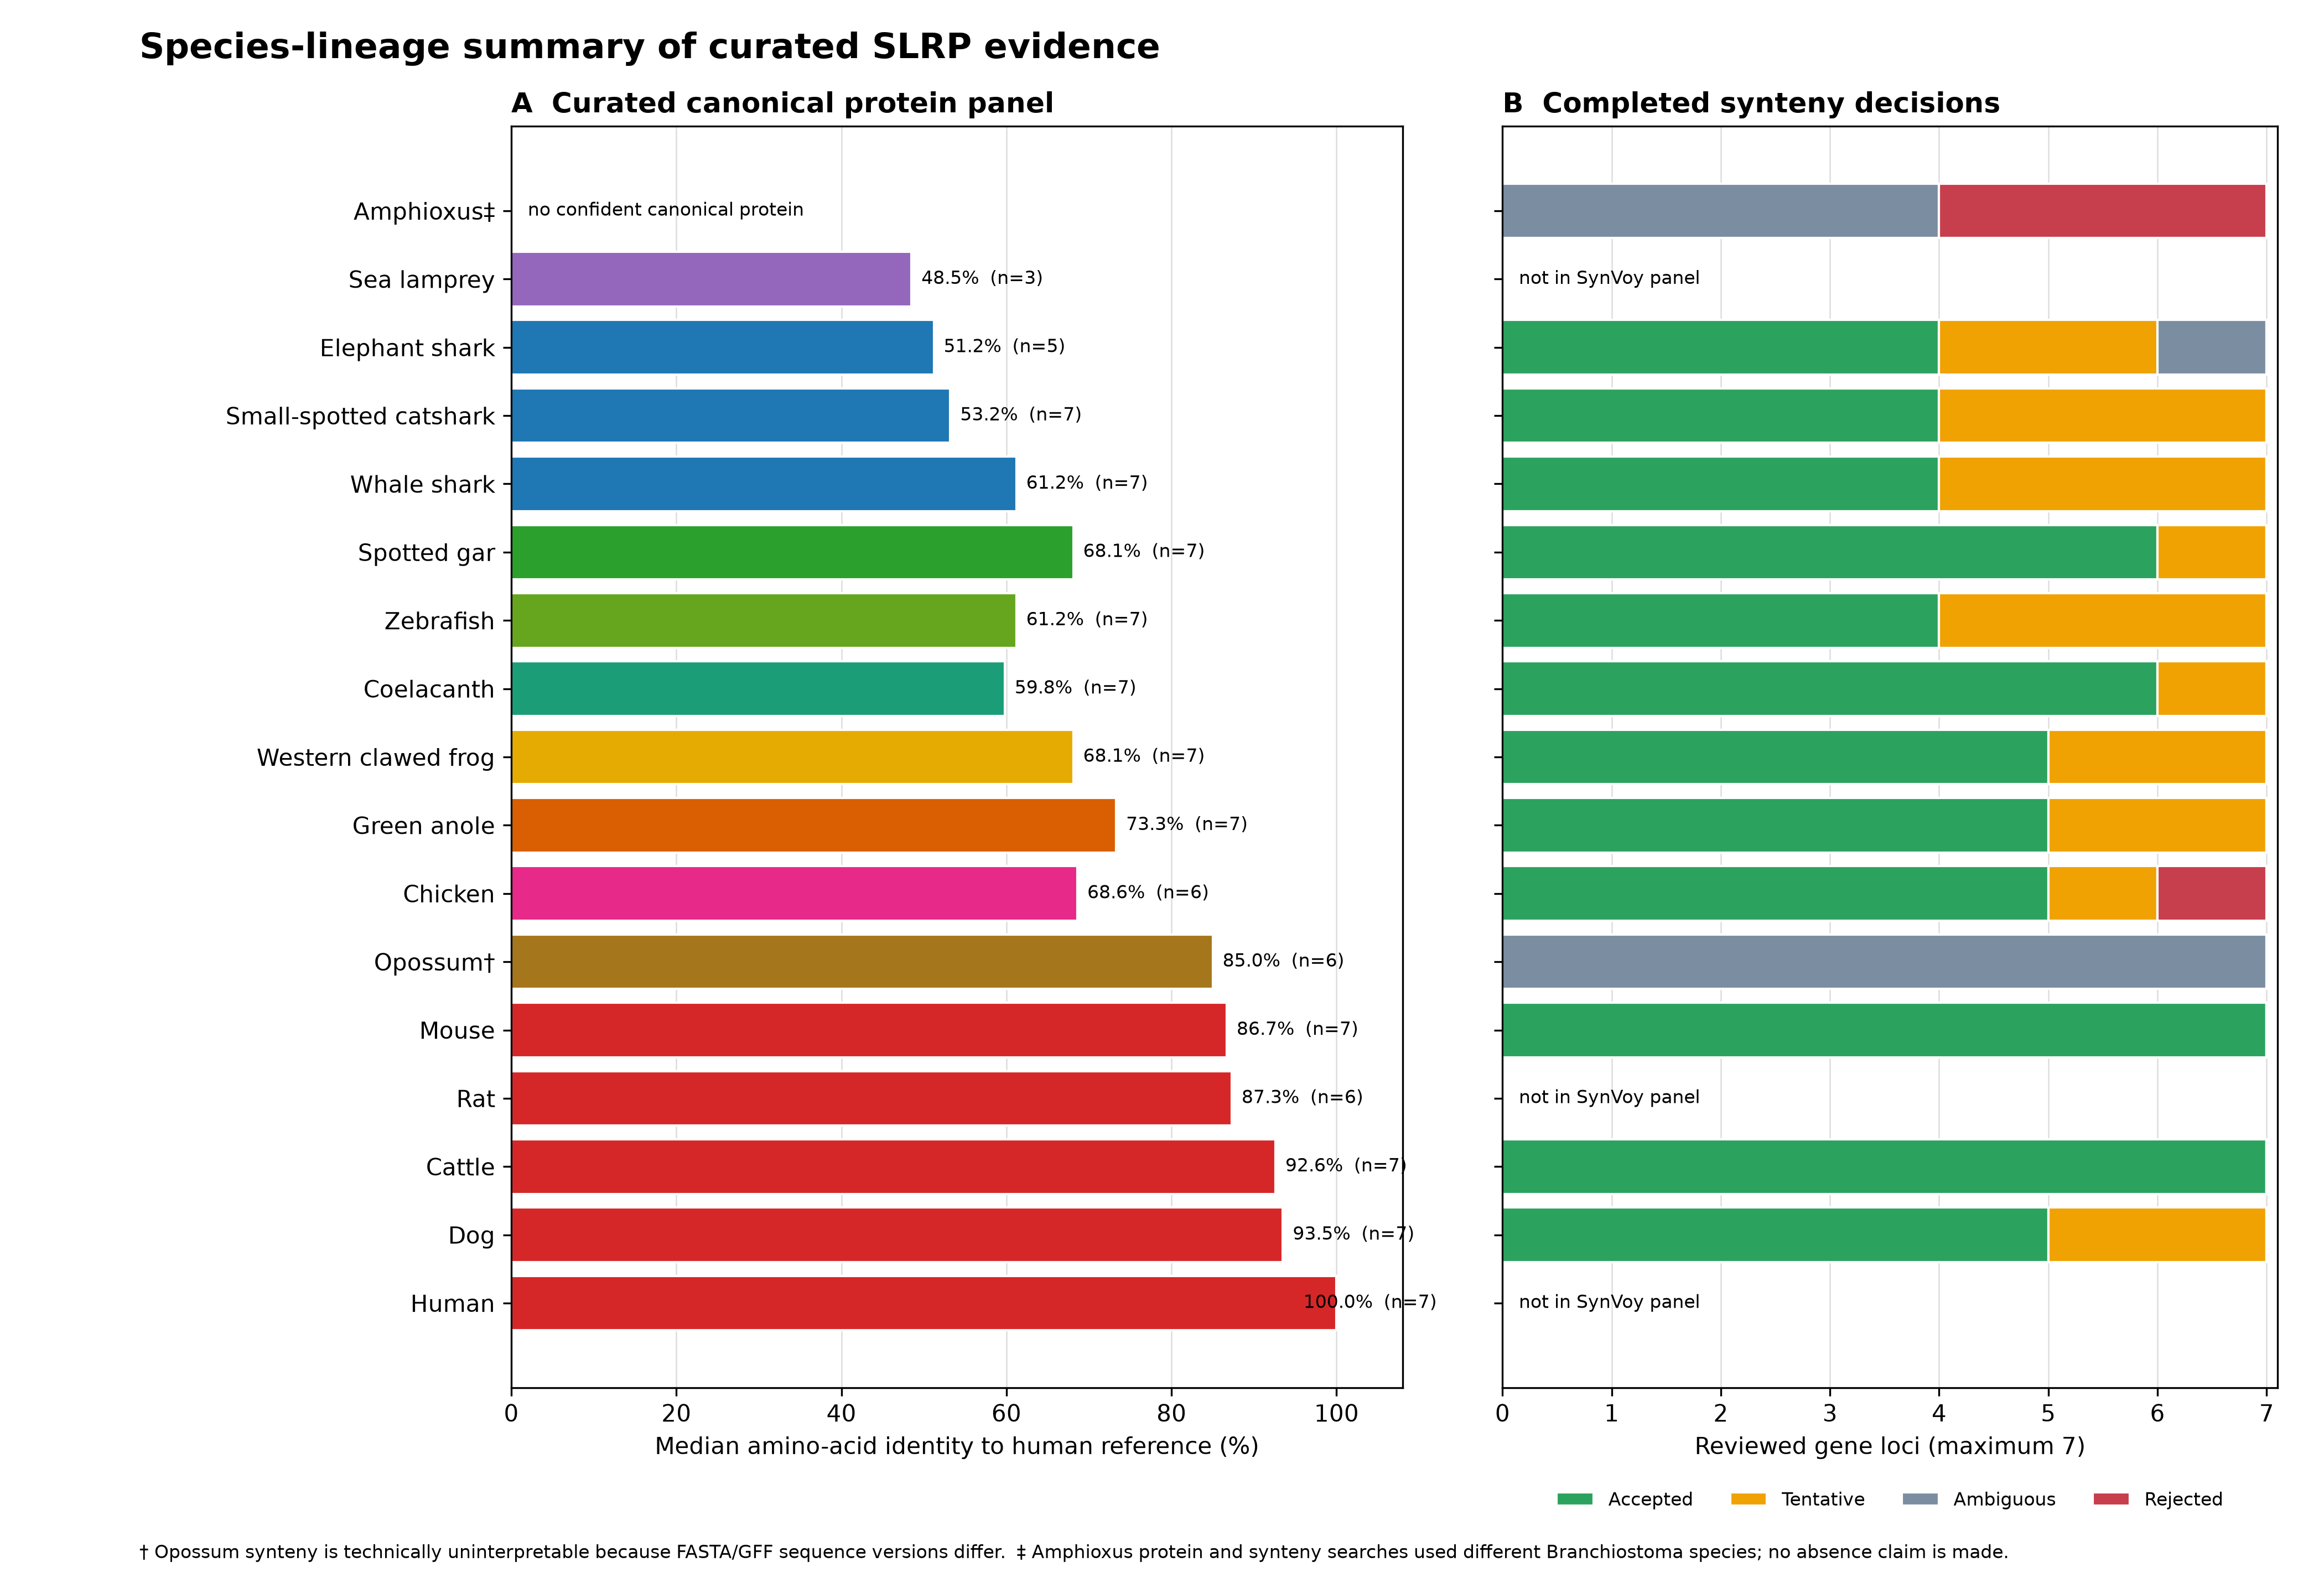
\includegraphics[width=\textwidth]{figures/overview/species_lineage_evidence_summary.png}
    \caption[Species-lineage summary of curated SLRP evidence]{Species-lineage
    summary of the curated comparative evidence. (A) Median amino-acid identity
    to the human reference across the canonical proteins available for each
    species; labels give the number of retained proteins and bar colours denote
    lineage groups. Medians based on different gene subsets are descriptive and
    are not a molecular-clock analysis. (B) Recorded locus-audit decisions
    across the seven focal genes. Rat and lamprey were not SynVoy targets, and
    human supplied the home locus. Opossum calls are technically uninterpretable
    because the FASTA/GFF sequence versions differ. The amphioxus protein and
    synteny searches used different \textit{Branchiostoma} species, and absence
    of a confident candidate was not interpreted as gene loss.}
    \label{fig:species-lineage-summary}
\end{figure}

\subsection{Microsynteny and manual locus-review status}
\label{subsec:results-synteny}

Completed SynVoy reports for BGN, DCN, EPYC, FMOD, LUM, OGN, and PRELP were
parsed across 14 non-human target genomes, yielding a 98-row gene-by-genome
evidence table. The numbers of genomes with a best retained HIGH call were 9
for BGN, 10 for DCN, 9 for EPYC, 10 for FMOD, 10 for LUM, 13 for OGN, and 11
for PRELP. HIGH and MEDIUM values identify retained automated candidates, not
verified one-to-one orthologs, because one genome can contribute multiple calls
or a rescue-derived candidate. The automated results were therefore used to
locate and prioritize loci rather than as a binary orthology test.

The review scheme assigned 26 rows to detailed P1 feature and neighbourhood
inspection, 68 to rapid P2 accession--locus confirmation, and four to P3
controls. All 98 rows have a recorded evidence-based decision: 62 were
accepted, 20 retained as tentative, 12 remained ambiguous, and four were
rejected. These decisions include batch GFF/accession checks and should not be
read as 98 independent visual GDV confirmations. In 69 combinations,
the canonical protein accession directly overlapped the best post-ownership
SynVoy locus in the exact target GFF3, showing that the automated coordinate
and the protein analysed elsewhere represented the same model in those cases.

Detailed review showed why the remaining automated calls could not be read as
a one-to-one orthology table. Canonical EPYC in coelacanth, elephant shark and
spotted gar; LUM in catshark, coelacanth and spotted gar; and PRELP in zebrafish
were accepted using concordant locus, flanking-gene, protein and tree evidence.
The vertebrate \textit{EPYC--KERA--LUM--DCN} region was especially informative:
the corresponding block and several distal anchors remained ordered in
coelacanth, spotted gar and zebrafish even when SynVoy selected a different
fragment. By contrast, the amphioxus EPYC and FMOD intervals overlapped
unrelated RUN-domain- and BRD3-like genes, respectively, and the amphioxus OGN
raw calls were assigned to other genes. Chicken \texttt{XP\_414298.2} was also
rejected from BGN because its product, focused tree and locus neighbours were
ASPN-like.

The locus audit additionally resolved duplicated or annotation-sensitive FMOD
cases. In zebrafish, \textit{fmodb} was the better full-length human-FMOD match,
whereas \textit{fmoda} retained the ancestral FMOD--PRELP neighbourhood; both
were therefore retained as co-ortholog evidence. The updated-tool FMOD report
was integrated rather than treated as a pending rerun. It contained 10 HIGH and
five MEDIUM retained calls, compared with 12 HIGH and seven MEDIUM in the
historical report. Most changes did not alter the final biological decision,
but in spotted gar the updated best HIGH rescue directly overlapped canonical
\textit{fmoda}; eight shared human flanking genes independently supported that
locus. Amphioxus remained rejected, whereas catshark, whale shark, and
zebrafish retained qualified decisions based on the combined locus and protein
evidence rather than the automated rank alone. The elephant-shark
fibromodulin-like model remained
tentative despite a complete 684-aa translation from nine CDS segments. BLASTP
assigned residues 1--330 most strongly to DCN (47.0\% identity) and residues
376--684 most strongly to FMOD (57.0\% identity; 82.2\% coverage of human
FMOD). Pfam detected LRR architecture across both halves and separate LRR
N-terminal caps at residues 54--76 and 383--412. Together with a second
hydrophobic segment at residues 330--347, this supported a compound or fused
gene model rather than a confident single-copy FMOD protein. The locus was
retained as tentative FMOD evidence, but the protein was excluded from the
confident FMOD panel.

All seven opossum rows were classified as ambiguous for synteny because the
GFF3 and FASTA used for those completed reports had incompatible chromosome
sequence versions. A replacement GCF\_027887165.2 pair subsequently passed the
identifier audit, but its gene-level reruns were not complete at the data
freeze. This technical exclusion does not invalidate independently supported
opossum proteins, but it prevents use of the completed SynVoy scores as locus
evidence.
A gene absent from a retained SynVoy call was otherwise recorded as unresolved,
not as a demonstrated evolutionary loss. Figure~\ref{fig:synvoy-overview}
separates the automated call from the recorded integrated locus decision.

\begin{figure}[htbp]
    \centering
    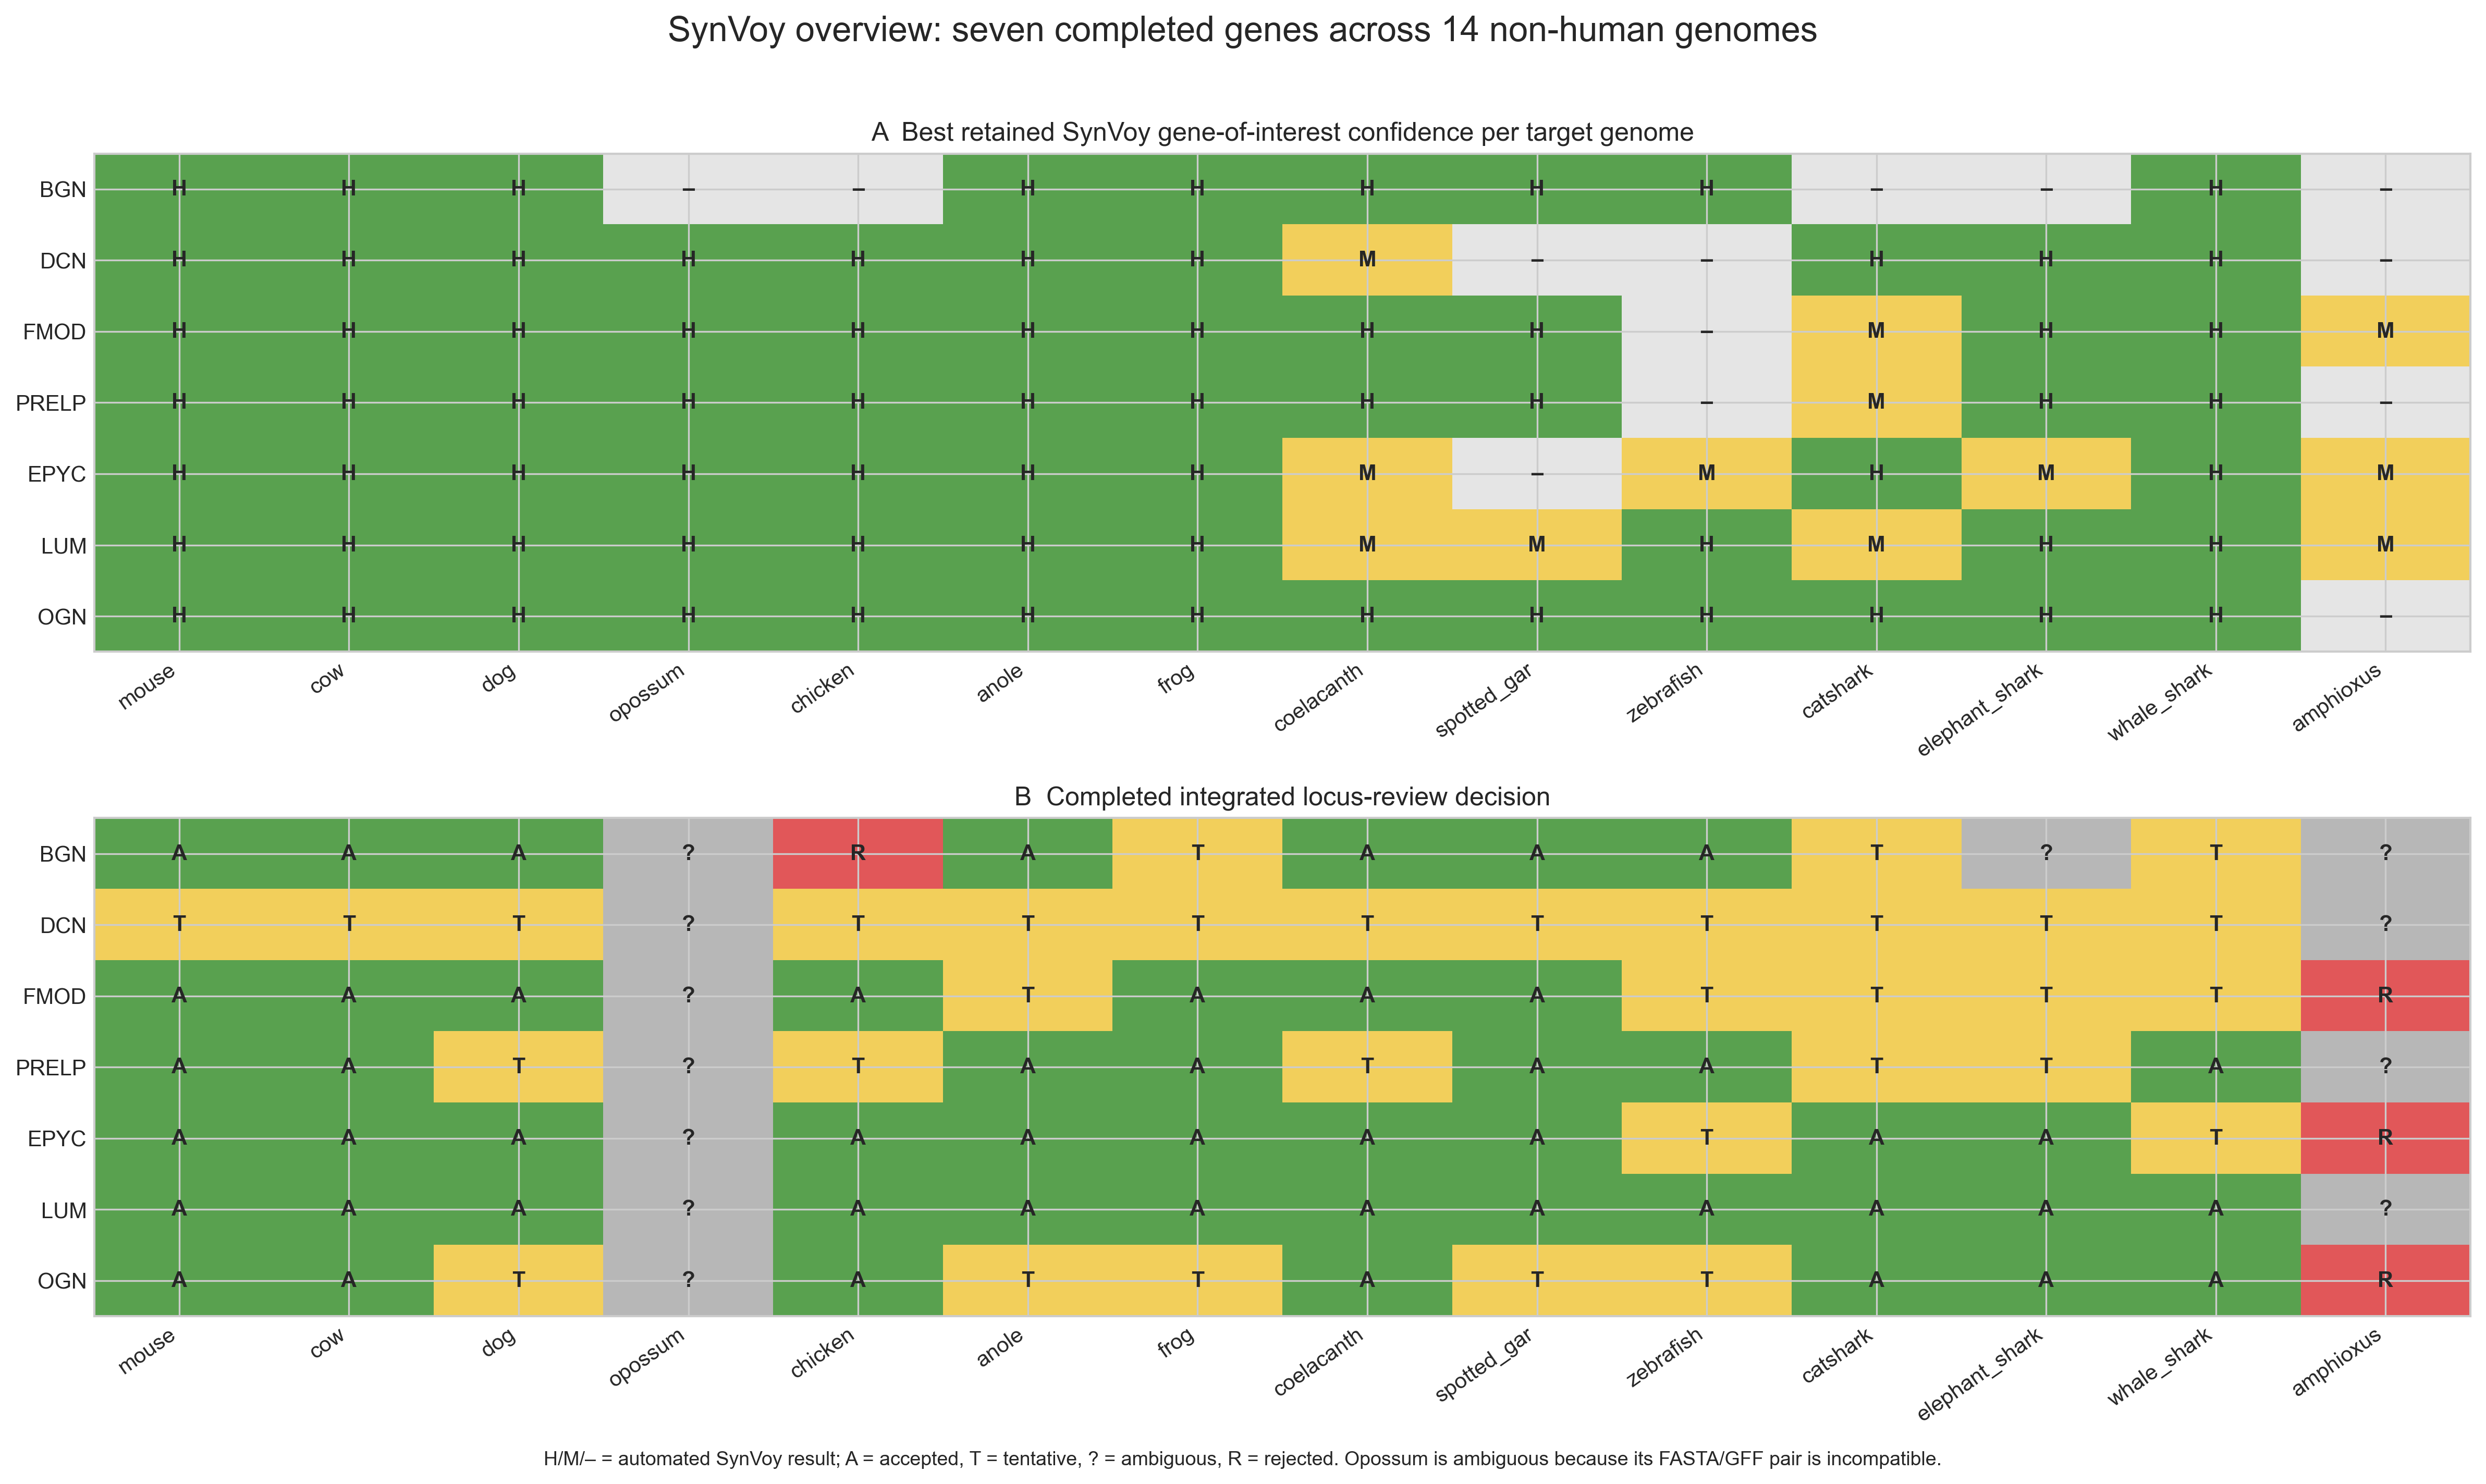
\includegraphics[width=\textwidth,height=0.76\textheight,keepaspectratio]
        {figures/synteny/synvoy_species_confidence_heatmap.png}
    \caption{SynVoy locus-level evidence and recorded review outcomes for seven
    genes across 14 non-human target genomes. Panel A shows the best retained
    automated candidate class after ownership/paralog filtering: H, HIGH; M,
    MEDIUM; dash, no retained HIGH/MEDIUM call. Panel B shows the integrated
    locus decision: A, accepted; T, tentative; question mark, ambiguous; R,
    rejected. Decisions combine exact-assembly GFF/accession checks with
    detailed review of prioritized exceptions; they are not 98 independent
    visual GDV confirmations. A missing automated call is not evidence of gene loss. All
    opossum outcomes are ambiguous because the target FASTA and GFF3 sequence
    identifiers were incompatible.}
    \label{fig:synvoy-overview}
\end{figure}

\subsection{Conserved coding organization and domain--exon architecture}
\label{subsec:results-gene-structure}

Representative protein-coding transcripts were compared for human, mouse, cow,
chicken, and zebrafish. Coding-exon number was constant across the five species
for each examined gene: seven CDS exons for BGN and DCN, six for EPYC and OGN, and two
for FMOD, PRELP, LUM, and OMD. Estimated protein lengths were correspondingly
stable, whereas total gene span varied more strongly because of intron-length
differences. No representative transcript was flagged as a structural outlier.
All 40 selected annotation models produced genome-reconstructed CDSs that were
divisible by three, began with methionine, contained a terminal stop codon, and
lacked internal stops; all coding blocks also passed their GFF phase-continuity
checks. These are annotation-quality results rather than automatic orthology
validation. The accession crosswalk identified 18 exact canonical-panel
accessions and 15 alternative accessions with equivalent or near-equivalent
translations. Zebrafish BGN structure was represented by \textit{bgna}, whereas
the canonical protein panel used \textit{bgnb}. The technically complete chicken
BGN-locus transcript encoded the ASPN-like product \texttt{XP\_414298.2} and was
therefore not counted as independent BGN orthology support. OMD remained a
five-species context-only comparison.

The higher-resolution splice analysis identified 26 coding junctions that were
comparable across all five species. Intron phase was conserved for all 26.
Exact boundary positions were especially close for BGN, for which all six
junctions varied by at most three amino acids, and for the single OMD junction,
which varied by two amino acids. The remaining genes preserved phase despite
modest boundary displacement (median gene-level ranges of 6--18 amino acids).
Thus, the shared exon counts represent a conserved frame-compatible coding
organization rather than only the same number of annotated boxes.
For BGN, this statement describes the selected annotated BGN-like/co-ortholog
set and does not override the chicken product conflict or the zebrafish
\textit{bgna}/\textit{bgnb} distinction.

The annotation-level isoform screen identified coding alternatives that could
change CDS-exon count and/or protein length at 11 of 40 loci. These flags were
concentrated in BGN (mouse and zebrafish), FMOD (zebrafish), PRELP (chicken),
EPYC (human, chicken, and zebrafish), LUM (cow), and OGN (human and zebrafish).
They identify transcript-choice sensitivity rather than representative-model
failure; all selected models passed the sequence-completeness checks. Full UTR
lengths varied much more than the coding organization and were therefore kept
as annotation-sensitive descriptive data. This conserved coding organization
supported stable gene models, but was interpreted together with protein, tree,
domain, and locus evidence rather than as stand-alone proof of orthology.

The representative-protein Pfam rescan recovered significant LRR-family
support in all 40 translations (294 significant repeat/domain hits in total).
At least one LRR-family model crossed a coding-exon boundary in representatives
of BGN, FMOD, PRELP, EPYC, LUM, and OGN; OMD hits remained within one coding
exon. The human domain--exon map therefore shows that the LRR-rich architecture
is generally distributed across the conserved coding framework rather than
being encoded as one independent exon-level module. The cross-species overview
in Figure~\ref{fig:gene-structure-overview} focuses on conserved coding
organization and distinguishes it from more variable total gene span.

\begin{figure}[p]
    \centering
    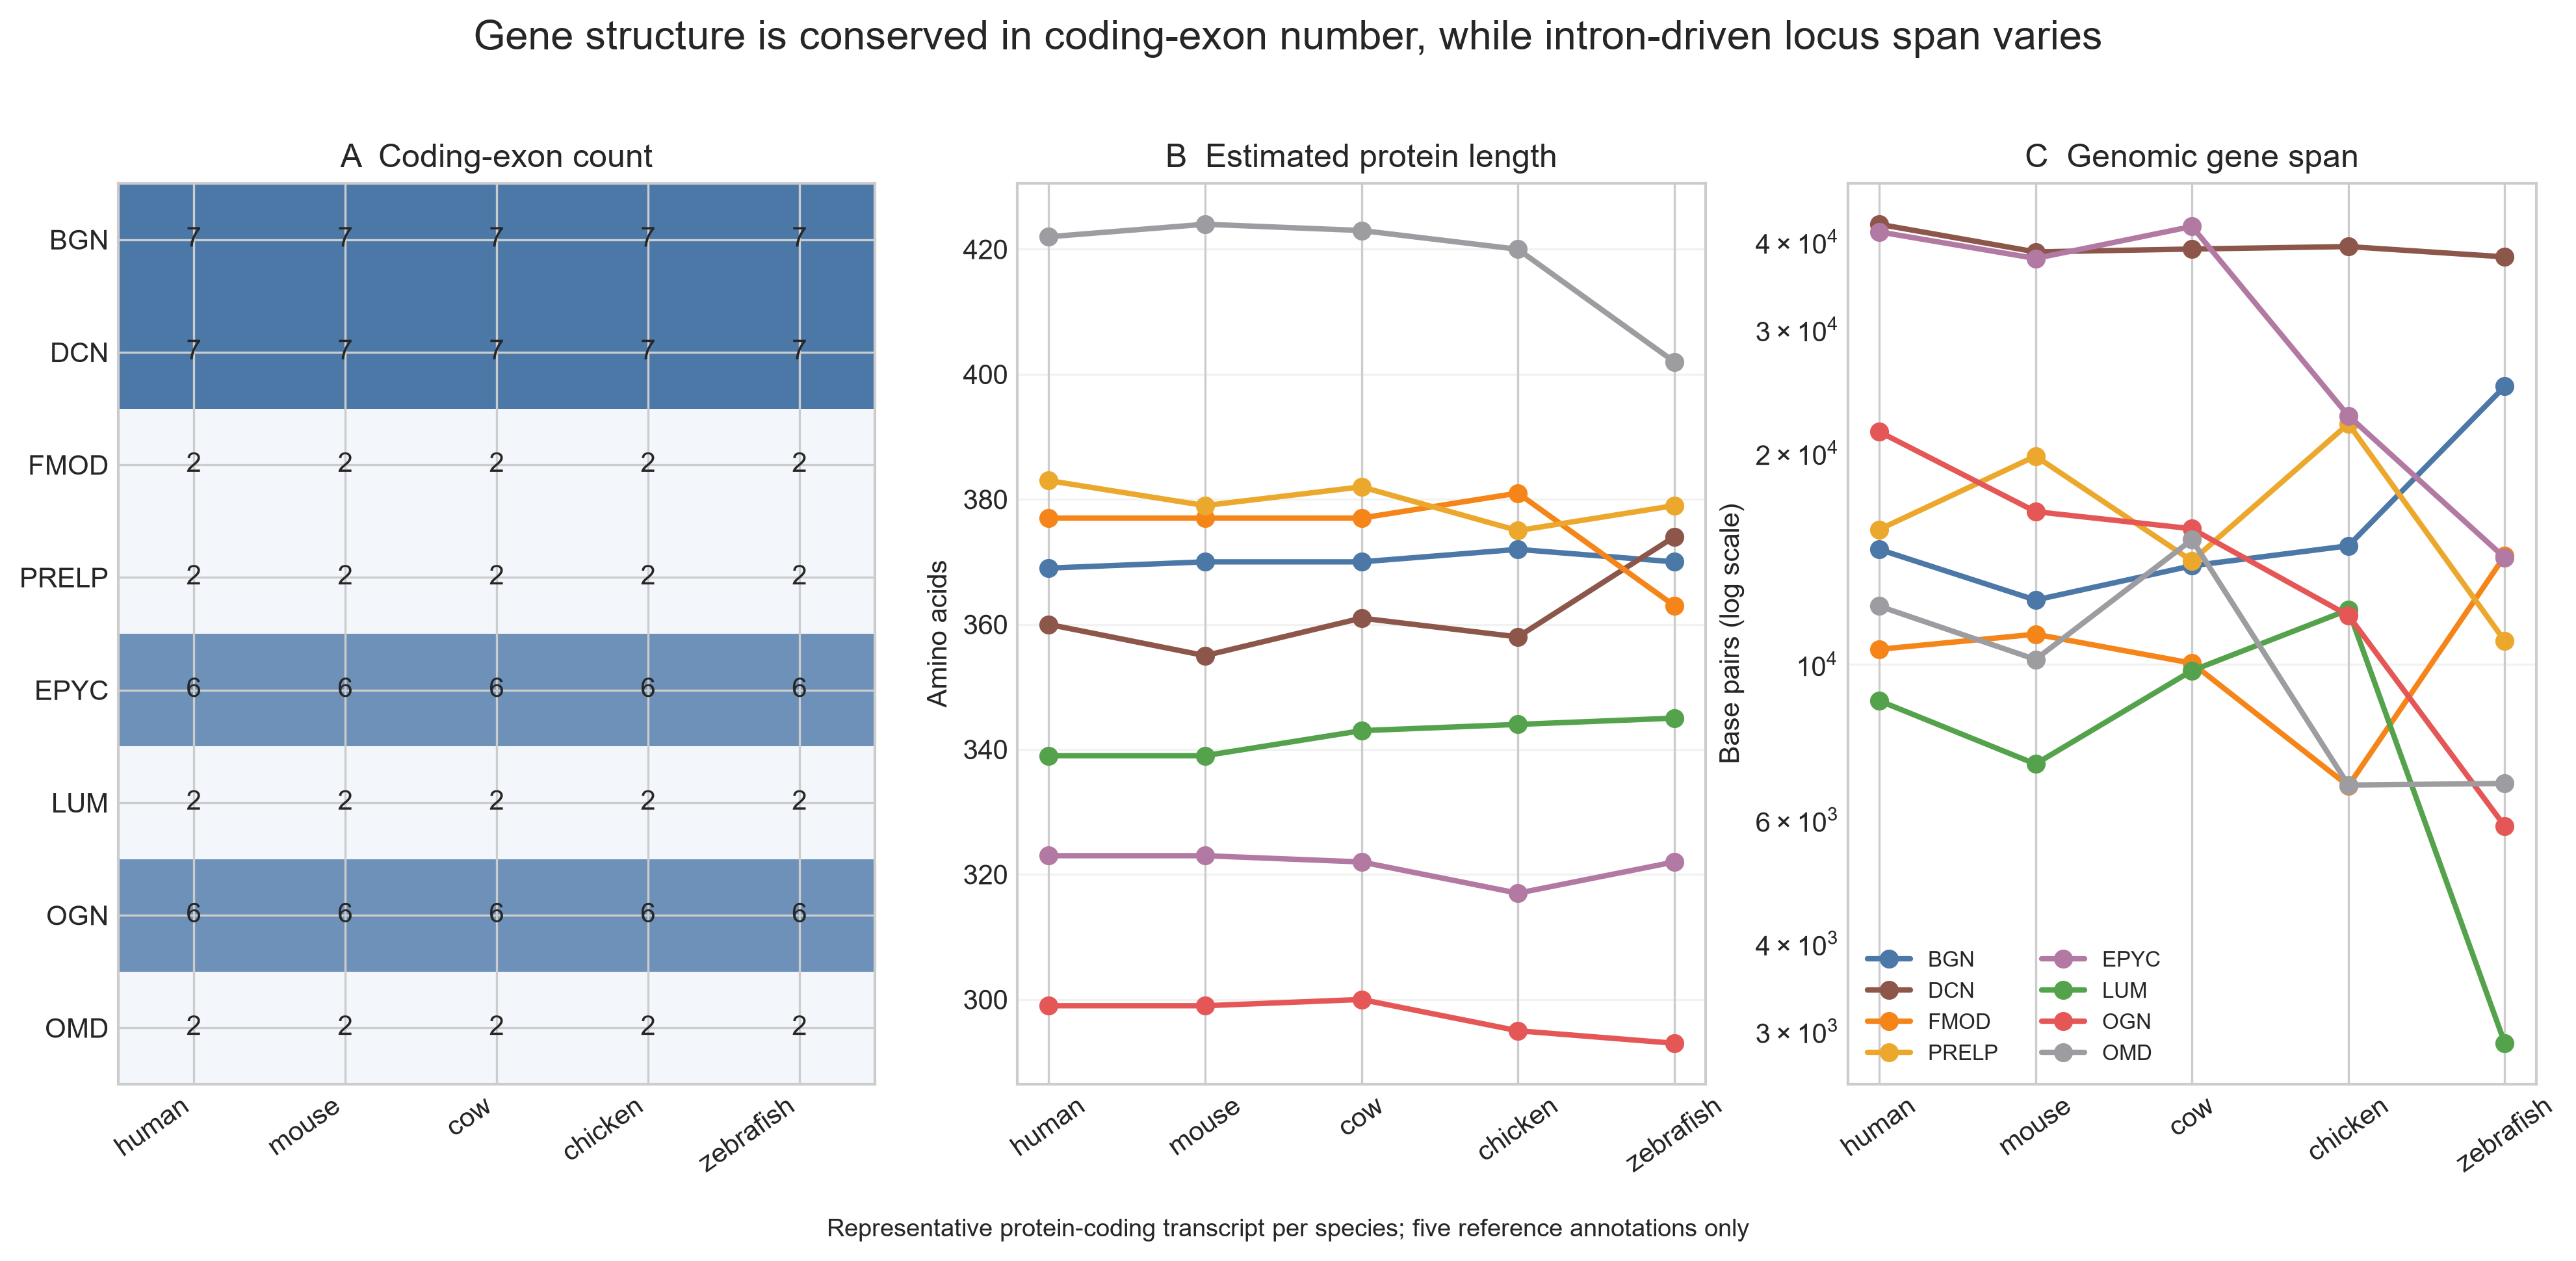
\includegraphics[width=\textwidth,height=0.82\textheight,keepaspectratio]
        {figures/gene_structure/gene_structure_conservation_overview.png}
    \caption{Conservation of representative protein-coding gene structure in
    human, mouse, cow, chicken, and zebrafish. Coding-exon number is stable
    within each of the seven comparative genes and OMD context, and estimated
    protein length is much more stable than intron-dependent genomic span.
    Results depend on the selected representative annotation and support gene-
    model plausibility rather than orthology by themselves. The chicken BGN
    annotation is structurally coherent but its product is ASPN-like, and the
    zebrafish BGN structure row represents \textit{bgna} rather than the
    canonical-panel \textit{bgnb}.}
    \label{fig:gene-structure-overview}
\end{figure}

\subsection{Supplementary coding-sequence constraint}
\label{subsec:results-codon-constraint}

Twenty-five of the 32 possible human--target NG86 comparisons produced a finite
$d_N/d_S$ estimate after excluding the ASPN-like chicken BGN-locus product.
Every interpretable ratio was below one (range 0.031--0.240), consistent with
predominant purifying constraint on these representative coding sequences.
Six human--zebrafish comparisons had undefined or non-positive $d_S$
and were not interpreted; PRELP was the exception ($d_N/d_S=0.203$).
Human--chicken EPYC and LUM also remained below one but had $d_S>2$ and were
flagged for possible synonymous-site saturation. The analysis therefore adds a
nucleotide-level constraint check for shallow and moderate comparisons, while
deep vertebrate comparisons remain outside its reliable range.

\subsection{Curated mouse and human phenotype evidence}
\label{subsec:results-phenotypes}

The MGI analysis recovered 118 focal records and 105 unique
gene--Mammalian-Phenotype-term--evidence combinations; all recovered focal
records represented single-gene genotypes in the downloaded release. BGN had
19 unique phenotype terms, including 14 skeletal/cartilage/joint terms; DCN had
24 terms, including 4 in that category; FMOD had
8 terms, including 4 in that category; and EPYC had 3 terms, including short
femur and osteoarthritis. LUM had 31 terms dominated by corneal and
skin/connective-tissue phenotypes, with one tendon-related skeletal term. OGN
had 8 terms dominated by corneal, collagen/skin, cardiovascular, and metabolic
annotations. PRELP had 12 terms but no term assigned to the broad
skeletal/cartilage/joint category in this release.

The pinned HPO release contained 89 focal gene--phenotype rows: 79 for BGN and
10 for DCN. It linked BGN to Mendelian OMIM:300106 and OMIM:300989 and DCN to
OMIM:610048. The absence of HPO rows for the other five genes was treated as a lack of curated human
disease annotation in that release, not as evidence of absent biological
function. Because phenotype-database counts depend on study and curation depth,
they were not used to rank candidate importance.

\subsection{Supplementary mature-protein motif analysis}
\label{subsec:results-protein-motifs}

MEME identified recurrent sequence blocks in the mature-protein proxies: 37
motifs in the combined 103-protein panel and 79 motifs across the seven separate
gene models; STREME returned 35 gene-enriched patterns. Signal peptides were
removed from all 100 SignalP-positive proteins, whereas the three
SignalP-negative proteins remained untrimmed. The motifs were dominated by
conserved LRR-rich and
cysteine-rich sequence blocks and were therefore interpreted as sequence
conservation rather than as experimentally established functional sites.

When every protein was scanned against all seven gene-specific motif models,
all 103 proteins scored most strongly against the model learned from their
assigned gene. Thus, the motif analysis supplied no new candidate outlier. It
added classification support to the curated assignments but did not remove
independent reciprocal-hit, coverage, partial-model, or SignalP caveats. Because
the same small curated sets were used to learn and evaluate the models and no
independent hold-out was available, this was not treated as an independent
accuracy estimate.

\subsection{Supplementary exploratory promoter analysis}
\label{subsec:results-promoter-motifs}

Seventy strand-aware promoter sequences were extracted from 35 representative
loci: core and proximal windows for each of seven genes in human, mouse, cow,
chicken, and zebrafish. All sequences had their expected length, none was
clipped at a contig edge, and none contained ambiguous bases. Proximal-promoter
GC content ranged from 32.48\% to 59.06\%.

No site from the targeted 40-profile transcription-factor panel passed the
strict FIMO threshold of $q\leq0.05$, and no targeted motif reached the
panel-corrected AME threshold of $E<0.05$. HIF1A was the strongest targeted AME
result (raw $p=7.49\times10^{-5}$; within-motif adjusted $p=0.0638$), but its
panel-corrected E-value was 2.55. Twelve motifs from the full JASPAR collection
passed $E<0.05$; several were A-rich, T-rich, or repetitive, as were many global
de-novo motifs. The analysis therefore did not identify a statistically
supported shared cartilage/growth-plate regulatory signature. Uncorrected
cross-species recurrences were retained only as hypotheses for future
chromatin-occupancy or reporter experiments.

\subsection{Integrated gene-level interpretation}
\label{subsec:results-gene-specific-summary}

BGN and FMOD provided the strongest combined expression and technical anchors.
DCN contributed direct cartilage/ECM support and the essential class-I paralog
control that exposed contaminated BGN assignments.
PRELP was strongly supported by the direct zone-resolved growth-plate dataset
despite only moderate abundance in the broader P0 lineage sample. EPYC had lower
RNA abundance but a direct anatomical rationale and coherent comparative
evidence. LUM had a clean protein and gene-structure profile; manual locus
review accepted its canonical catshark, coelacanth, and spotted-gar loci despite
different SynVoy-selected fragments, while amphioxus remained unresolved. OGN contributed evolutionary and
class-III breadth but remained the least certain growth-plate candidate; its
final vertebrate set was coherent only after exclusion of the amphioxus
SLRP-like sequence and tentative treatment of spotted gar.
Figure~\ref{fig:integrated-evidence} places these gene-level findings side by
side while preserving the original units and caveats of each evidence layer.

\begin{figure}[p]
    \centering
    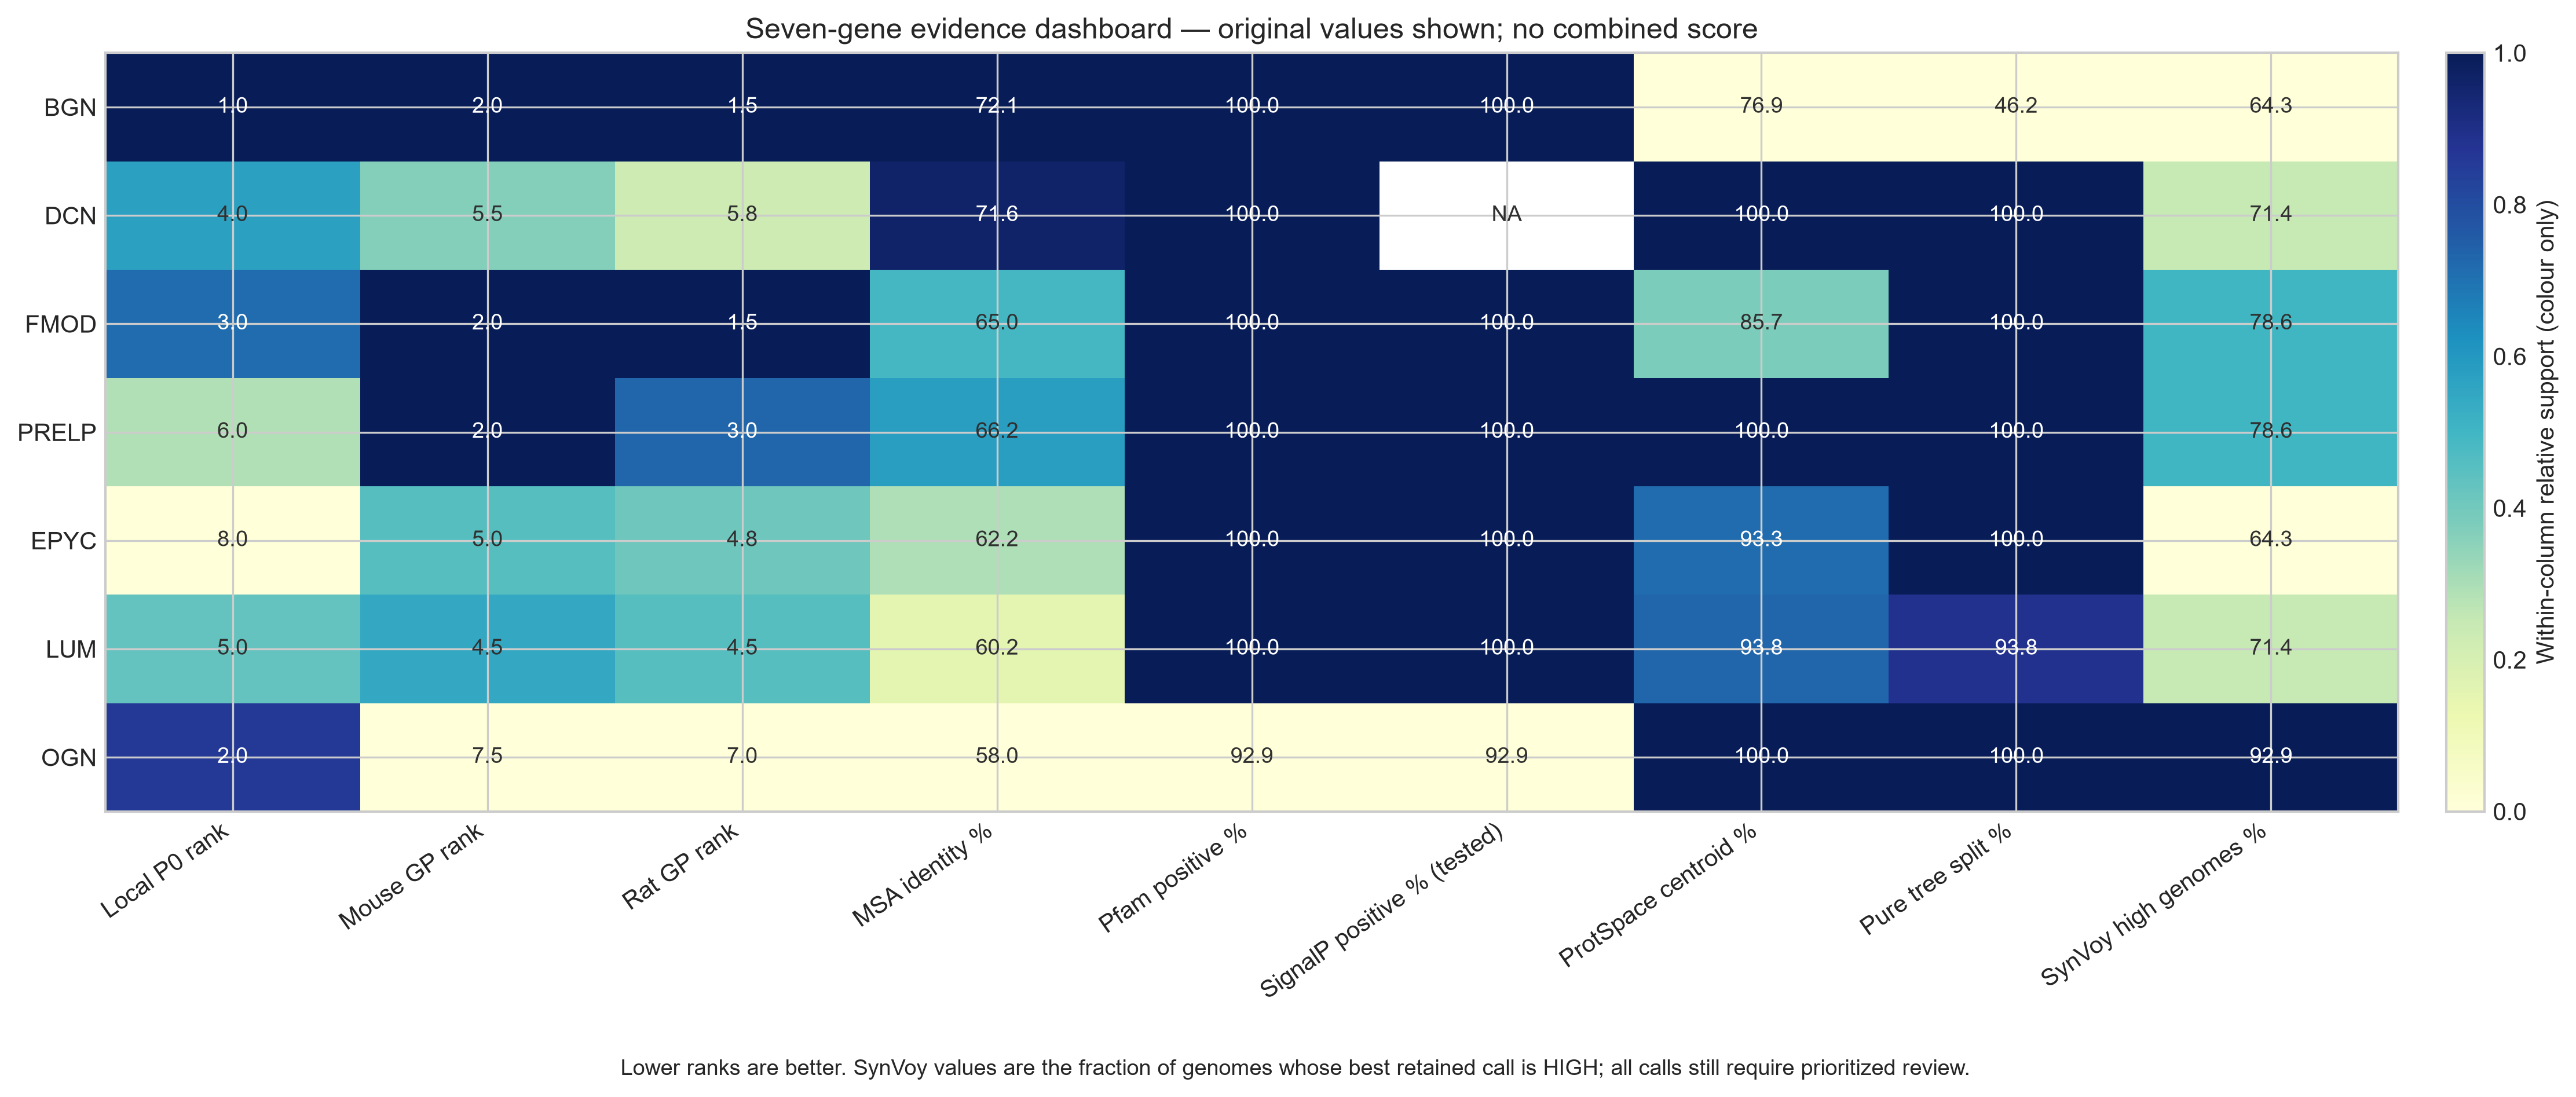
\includegraphics[width=\textwidth,height=0.82\textheight,keepaspectratio]
        {figures/overview/integrated_evidence_dashboard.png}
    \caption{Integrated evidence summary for the seven-gene comparative panel.
    Expression, protein/domain, phylogenetic, synteny, gene-structure, motif,
    and phenotype evidence retain their original units and limitations; panel
    colours are normalized within evidence types and are not combined into an
    unsupported numerical confidence score.}
    \label{fig:integrated-evidence}
\end{figure}


\newpage
\section{Discussion}
\label{sec:discussion}
% ============================================================
% Discussion draft generated from the integrated evidence package.
% ============================================================

\subsection{Conservation supports a shared extracellular-matrix framework}
\label{subsec:discussion-main-findings}

The main result is not simply that the selected genes are ``highly conserved.''
Rather, several independent evidence types converge on a conserved molecular
framework: most candidates retain a secretion signal, SLRP/LRR-family
architecture, a continuous conserved alignment core, stable CDS-exon
organization, gene-specific phylogenetic placement, and---where SynVoy is
complete---locus-level support. This combination is consistent with long-term
maintenance of secreted extracellular-matrix proteins while allowing divergence
in terminal regions, individual repeats, expression level, and lineage-specific
gene history.

This interpretation agrees with the broader view of SLRPs as both structural
matrix organizers and regulators of receptor or growth-factor signalling
\citep{SchaeferIozzo2008,IozzoSchaefer2015}. A conserved N-terminal signal
peptide supports entry into the secretory pathway and therefore compatibility
with extracellular localization. Conserved LRR-rich architecture supports SLRP
family identity and preservation of a protein-interaction scaffold. Neither
feature proves that every ortholog binds the same partner or has the same
phenotype, but their joint conservation makes a conserved extracellular role
biologically plausible.

\subsection{Gene-specific relevance to cartilage and the growth plate}
\label{subsec:discussion-biological-relevance}

BGN and FMOD are the strongest anchors because their high juvenile and
growth-plate expression is accompanied by skeletal functional evidence. In mice,
combined Bgn/Fmod deficiency alters bone mass and osteoclastogenesis, and both
proteins interact with regulators of osteoclast formation \citep{Kram2017}.
FMOD is additionally localized around late-hypertrophic chondrocytes, the
secondary ossification centre, and the growth plate during knee development
\citep{Saamanen2001}. Their strong protein, tree, and gene-structure support is
therefore consistent with conserved roles at the interface between collagen-rich
matrix organization and skeletal remodelling. DCN adds a closely related class-I
comparison with direct collagen-fibril, cartilage-pericellular-matrix, and
mechanotransduction evidence. Its inclusion was methodologically important
because reciprocal comparison against DCN exposed several historical BGN
misassignments. Conserved DCN domains, alignment, tree placement, coding
organization, phenotype annotations, and the completed updated SynVoy run
support its inclusion. The completed SignalP screen detected a classical signal
peptide in 14 of 15 DCN proteins. The only negative, opossum
\texttt{XP\_001363160.3}, is a C-terminal fragment missing the corresponding
N-terminal region and therefore does not argue against secretion of intact DCN.

The FMOD locus results also illustrate a biologically meaningful consequence
of teleost duplication. Zebrafish \textit{fmodb} provided the more complete
human-FMOD sequence match, whereas \textit{fmoda} retained the ancestral
FMOD--PRELP neighbourhood. Spotted-gar \textit{fmoda} was likewise supported by
an alternative retained SynVoy locus and eight shared human flanking genes,
even though the run summary ranked a nearby lumican-like/PRELP interval first.
These cases support retention of duplicated co-ortholog evidence rather than
forcing every species into a single best-hit model. The elephant-shark FMOD-
like locus remains tentative because its reconstructed 684-aa product contains
two SLRP-like halves. Protein BLAST assigned the N-terminal half most strongly
to DCN and the C-terminal half most strongly to FMOD; two LRR N-terminal caps
and a second hydrophobic segment near residue 330 further support a compound or
fused gene model. The locus is informative, but this protein was therefore not
included in the confident FMOD sequence panel.

PRELP illustrates why candidate selection should not be reduced to one RNA
ranking. Its abundance in the broad P0 lineage sample was moderate, whereas the
direct mouse and rat growth-plate data were strong. PRELP is a cartilage matrix
protein with conserved LRR and cysteine-containing regions
\citep{Grover1996,Grover2002}; its N-terminal region and full-length protein have
also been linked to osteoclast and osteoblast regulation
\citep{Rucci2009,Li2016PRELP}. The highly conserved protein and compact
two-CDS-exon organization found here give molecular context to those reported
skeletal functions.

EPYC provides a biologically specific class-III example. Its expression was not
among the highest in the initial screen, but developmental data place EPYC in
the extracellular matrix surrounding resting, proliferating, and hypertrophic
growth-plate chondrocytes \citep{Johnson1999}. Thus, the conserved EPYC protein
architecture and phylogenetic assignment are relevant to a protein with direct
growth-plate localization. The whale-shark sequence was retained as tentative
because its conserved middle-to-C-terminal region supports EPYC identity while
earlier mismatches, reduced coverage, and an alternative reciprocal hit leave
model uncertainty.

LUM combines consistent rodent expression with a technically clean vertebrate
protein set. Experimental studies connect lumican to skeletal matrix development
and cartilage collagen deposition and fibrillogenesis
\citep{Raouf2002,Kafienah2008}. The conserved signal peptide and LRR-rich core
therefore fit a secreted collagen-associated ECM role. Nevertheless, the
lamprey placement shows that close class-II SLRP paralogs can be difficult to
separate in deep lineages. The completed LUM SynVoy run recovered best HIGH
calls in 10 of 14 targets and MEDIUM calls in four. Manual review accepted the
canonical catshark, coelacanth, and spotted-gar LUM loci because their ordered
flanking blocks agreed with reciprocal protein and tree evidence, even though
the automated summary selected different fragments. Amphioxus remained
ambiguous because its candidate interval was intergenic and lacked an
independent canonical protein. Thus, manual review refined the automated result
rather than converting all 14 targets into proven one-to-one orthologs.

OGN is scientifically useful precisely because its evidence is less uniform.
OGN processing affects its regulation of type-I collagen fibrillogenesis
\citep{Ge2004}, while vertebrate analyses document teleost duplication and
subfunctionalization \citep{Costa2018}. Those observations explain why a
divergent zebrafish protein can still be a credible OGN-family ortholog, but they
do not validate the amphioxus sequence. Excluding amphioxus from the confident
set was justified by the combination of divergent terminal structure, large
sequence-specific insertions, an alternative reciprocal hit, poor synteny, and
its position outside the former main OGN split. Spotted-gar OGN remains a more
limited uncertainty: its LRR-rich alignment is plausible, but the absence of a
SignalP-positive N terminus prevents a fully confident secretion claim.

OMD should be discussed as supporting context rather than silently promoted to
the same evidential level as the seven-gene panel. OMD is secreted by osteoblasts,
binds mineral, supports osteoblast attachment, and occurs in fetal
growth-plate-associated primary spongiosa \citep{Sommarin1998}. It has also been
linked to BMP2/SMAD osteogenic signalling through terminal LRR interactions
\citep{Lin2021OMD}. These findings make OMD relevant to the cartilage--bone
interface, but its full cross-species protein, phylogenetic, and synteny pipeline
was not performed here.

\subsection{Why comparative evolutionary analysis remains informative}
\label{subsec:discussion-evolution-orthology}

Strong conservation does not make the comparative analysis uninformative. It
establishes which molecular features are maintained, exposes lineage-specific
exceptions, and identifies annotation or orthology errors that a single BLAST
hit would miss. In this dataset, the analysis resolved an ASPN-like chicken
BGN-locus product, removed an uncertain amphioxus OGN sequence, retained a
divergent but structurally coherent zebrafish OGN, and isolated deep-lineage
cautions for spotted-gar OGN and lamprey LUM. These exceptions are more
biologically informative than a blanket statement that all sequences are
conserved.

The deep-lineage sampling also places these gene-level observations in the
published history of SLRP evolution. Tunicate SLRP-like genes provide
literature-only precursor context, while the diversification reported in
jawless vertebrates and the recognizable repertoire in cartilaginous fishes
support expansion of the family during early vertebrate evolution
\citep{Park2008,Costa2018}. The present data do not reconstruct ancestral
sequences or date individual duplications. They instead test whether modern
gene-specific assignments remain recognizable across this evolutionary
bracket. The uncertain amphioxus OGN-like candidate, tentative lamprey LUM, and
partial shark BGN models define the empirical limit of that assignment.

The species-level measurements further show why evolutionary distance and
annotation quality must be separated. Median protein identity generally rose
from jawless/cartilaginous fishes toward mammals, but spotted gar exceeded both
zebrafish and coelacanth in the descriptive median and retained five of seven
reviewed loci. Conversely, opossum proteins were relatively close to human
while every opossum synteny row was unusable because of an input-version
mismatch. Thus, low confidence in a species cannot automatically be attributed
to biological divergence, and high protein identity cannot rescue invalid
locus data. The gar--zebrafish comparison is particularly informative because
gar brackets the ray-finned vertebrate condition before teleost-specific
duplication, whereas the two zebrafish FMOD co-orthologs expose that later
duplication history.

The evidence types answer different questions. Domain architecture supports
SLRP-family membership, phylogenetic clustering supports gene-specific
assignment, conserved coding-exon organization supports gene-model plausibility,
and synteny supports locus-level continuity. Agreement among them increases
orthology confidence; disagreement identifies cases for manual review. A
two-dimensional ProtSpace projection was used only as exploratory quality
control because visual proximity in an embedding cannot by itself establish
orthology.

The extended gene-structure analysis strengthens this conclusion beyond exon
count. Conservation of intron phase at all 26 comparable coding junctions means
that splice boundaries preserve their relationship to the reading frame even
where the exact boundary moved by several residues. Together with complete,
stop-free reconstructed translations, this is strong evidence for stable coding
models and homologous gene organization. It does not imply that UTRs or isoform
usage are conserved: those features varied more strongly and depend on
annotation and tissue-specific transcript use.

The supplementary pairwise $d_N/d_S$ analysis provides a complementary
nucleotide-level view. All finite estimates were below one, which is compatible
with predominant purifying constraint and fits the conserved protein cores.
However, the many unavailable human--zebrafish estimates and the high-$d_S$
bird comparisons show why this result cannot be generalized into a claim of
uniform selection across all vertebrate branches. A branch-aware codon model on
a carefully curated ortholog set would be required for formal lineage- or
site-specific selection inference.

\subsection{What the supplementary motif and phenotype analyses add}
\label{subsec:discussion-supplementary-evidence}

The mature-protein motif analysis reinforces, but does not replace, the MSA and
phylogenetic results. Every canonical protein was most compatible with the motif
model learned from its assigned gene, including the manually reviewed tentative
records. This is useful evidence that those sequences preserve gene-associated
patterns across the mature protein. However, many recovered patterns overlap
the expected LRR- and cysteine-rich architecture. Without biochemical testing,
they should not be assigned a specific collagen-binding, receptor-binding, or
signalling function.

Curated mutant and disease annotations add an independent bridge from molecular
conservation to organismal biology. The concentration of skeletal, cartilage,
or joint terms for BGN, DCN, FMOD, and EPYC is consistent with their main-panel roles.
The broader corneal, skin, tendon, and collagen phenotypes associated with LUM
and OGN support general ECM functions but do not demonstrate a growth-plate
phenotype. PRELP's lack of a skeletal-category MGI term in the downloaded
release does not contradict its direct growth-plate expression and experimental
literature. Annotation counts are strongly influenced by study effort and
database curation and therefore cannot be compared as gene-effect sizes.

The promoter analysis produced a biologically useful negative result. Despite
testing conserved de-novo patterns and a targeted cartilage/osteogenesis panel,
no targeted motif passed correction in this small five-species-per-gene design.
Promoter sequence alone therefore does not support a shared regulatory mechanism
for the seven genes. This does not weaken the protein-conservation conclusion:
regulatory conservation can occur in distal enhancers, in cell-state-specific
chromatin, or through turnover of individual motif instances. The uncorrected
recurrences are hypotheses that would require ATAC-seq, ChIP-seq, reporter
assays, or equivalent functional evidence.

\subsection{Limitations}
\label{subsec:discussion-limitations}

The initial P0 expression samples were developmentally relevant but not
microdissected growth-plate zones, while the direct GSE114919 dataset used a
different processed scale and a limited set of rodent ages and zones. Expression
therefore supports biological relevance, not gene function or causal importance.
Cross-species equivalence of expression was not tested by pooling these scales.

The comparative panel used 13--16 representatives per gene and
five reference species for the representative-transcript gene-structure screen.
Predicted proteins, incomplete assemblies, alternative isoforms, and errors in
gene naming can all affect candidate recovery. Conserved LRR domains also occur
across related SLRP paralogs, so domain similarity is not gene-specific proof.
The extended isoform inventory is annotation-based and does not identify the
dominant transcript in growth-plate cells. Derived UTR lengths are especially
sensitive to transcript-end annotation. Pairwise NG86 values average across a
whole sequence, and $d_S$ saturation made most human--zebrafish comparisons
uninterpretable; they are not evidence for branch- or residue-specific
selection.
The compact trees are unrooted; their split support does not establish the
direction or timing of duplication events. The completed SynVoy review showed
that rescue calls and genomes with no retained HIGH or MEDIUM candidate cannot
be interpreted without annotation and protein evidence. In addition, the
opossum FASTA/GFF sequence-version mismatch made all seven current opossum
synteny rows technically uninterpretable; these require a matched-input rerun.
Finally, computational conservation
supports compatibility with known functions but cannot demonstrate collagen
binding, signalling activity, or a growth-plate phenotype in each species.

The protein-motif models were learned and evaluated on the same compact
candidate panel, and the gene-level STREME comparisons had no independent
holdout set. The promoter analysis contained only five orthologous promoters per
gene, depended on one annotated transcription start site per locus, and did not
include distal enhancers or chromatin accessibility. MGI and HPO reflect
available genotype experiments and clinical curation rather than a standardized
phenotyping experiment across all seven genes. These supplementary layers are
therefore confirmatory or hypothesis-generating rather than decisive.

\subsection{Future directions}
\label{subsec:discussion-future-directions}

SignalP coverage and focused review of the partial BGN/DCN models are complete.
All 98 current SynVoy locus decisions are recorded: 62 are accepted, 20
tentative, 12 ambiguous and four rejected. The required synteny follow-up is a matched-input
opossum rerun; the interrupted updated-tool FMOD refresh and subsequent PRELP/
EPYC comparisons are optional sensitivity analyses if they remain in the final
scope. The tentative whale-shark EPYC sequence, duplicated zebrafish FMOD calls,
and tentative elephant-shark FMOD-like model should remain visible when the
evidence table is frozen. Broader expression work would be most valuable if it added matched
juvenile growth-plate zones or well-annotated single-cell data rather than simply
adding unrelated adult tissues. Regulatory follow-up should prioritize
growth-plate-relevant ATAC-seq/ChIP-seq or reporter data rather than another
larger sequence-only motif scan. Experimental protein work could test whether
the most conserved candidates retain collagen-, mineral-, or signalling-related
activities suggested by the literature.


\section{Conclusion}
\label{sec:conclusion}
This thesis established an expression-guided, multi-evidence framework for
evaluating seven cartilage- and growth-plate-relevant SLRPs across
representative vertebrates. BGN, DCN, FMOD, PRELP, EPYC, LUM, and OGN generally
retain a strongly conserved secreted LRR-rich protein core, and most assignments
are supported jointly by sequence alignment, domain architecture, gene-specific
phylogenetic placement, representative coding-exon organization, and genomic
neighbourhood. The seven completed SynVoy reports yielded a 98-row evidence
table, although 25 priority loci and subsequent rapid confirmations still
require manual biological review. BGN and FMOD are the strongest combined
biological and technical anchors; DCN is both a biologically supported candidate
and the essential class-I paralog control; PRELP, EPYC, and LUM remain well-
supported principal candidates; and OGN is most appropriately retained as an
exploratory vertebrate member.

Conservation was not uniform and did not make the comparative analysis
uninformative. The workflow exposed an ASPN-like chicken BGN-locus product,
excluded an amphioxus SLRP-like sequence from the confident OGN set, and retained
spotted-gar OGN, whale-shark EPYC, and lamprey LUM with explicit caveats. Stable
coding-exon counts coexisted with substantial intron-driven variation in locus
span, and mouse and rat growth-plate expression were not identical. These cases
show why orthology should be judged from concordant evidence rather than from a
gene label, one BLAST hit, or one conserved domain.

The evolutionary contribution is therefore not a claim that one sampled living
species represents the origin of an SLRP gene. Literature places an SLRP-like
precursor early in chordates and family expansion in early vertebrates. The
amphioxus--lamprey--cartilaginous-fish--bony-vertebrate bracket tested where
modern gene identities become confidently recognizable. The results support a
broadly established jawed-vertebrate SLRP repertoire while revealing decreasing
assignment certainty in the deepest lineages and in incomplete shark models.

Supplementary protein motifs supported every retained gene assignment, whereas
comparative promoter analysis did not reveal a corrected shared targeted
regulatory signature. Curated phenotype databases strengthened the skeletal
context of BGN, FMOD, and EPYC and provided broader ECM context for the other
genes, but did not justify ranking genes by annotation counts. Overall, the
results support evolutionary constraint on an extracellular-matrix SLRP toolkit
relevant to juvenile cartilage biology while clearly separating conserved
molecular compatibility from experimentally demonstrated growth-plate function
in each species. Targeted manual review of the prioritized ambiguous loci will
finalize the locus-level evidence layer.


\newpage
\section{Methods and Materials}
\label{sec:methods}
% ============================================================
% Materials and methods
% ============================================================

\subsection{Overview and evidence-integration strategy}
\label{subsec:workflow-overview}

The analysis combined independent evidence layers rather than treating any
single program as an orthology test. Juvenile skeletal and growth-plate
expression was used to prioritize biologically relevant small leucine-rich
proteoglycans (SLRPs). Candidate proteins were then evaluated by reciprocal
protein similarity, length and annotation checks, Pfam domain architecture,
signal-peptide prediction, multiple-sequence alignment, phylogenetic placement,
protein-language-model embeddings, conserved genomic neighbourhood, and
representative coding-gene structure. Conflicting or incomplete cases were
retained as tentative or excluded only after manual review of the combined
evidence. Exploratory protein-motif, promoter-motif, and phenotype-database
analyses were performed as supplementary validation; they were not used as
stand-alone candidate-selection criteria. The complete decision workflow is
summarized in Figure~\ref{fig:workflow-overview}.

\begin{figure}[htbp]
    \centering
    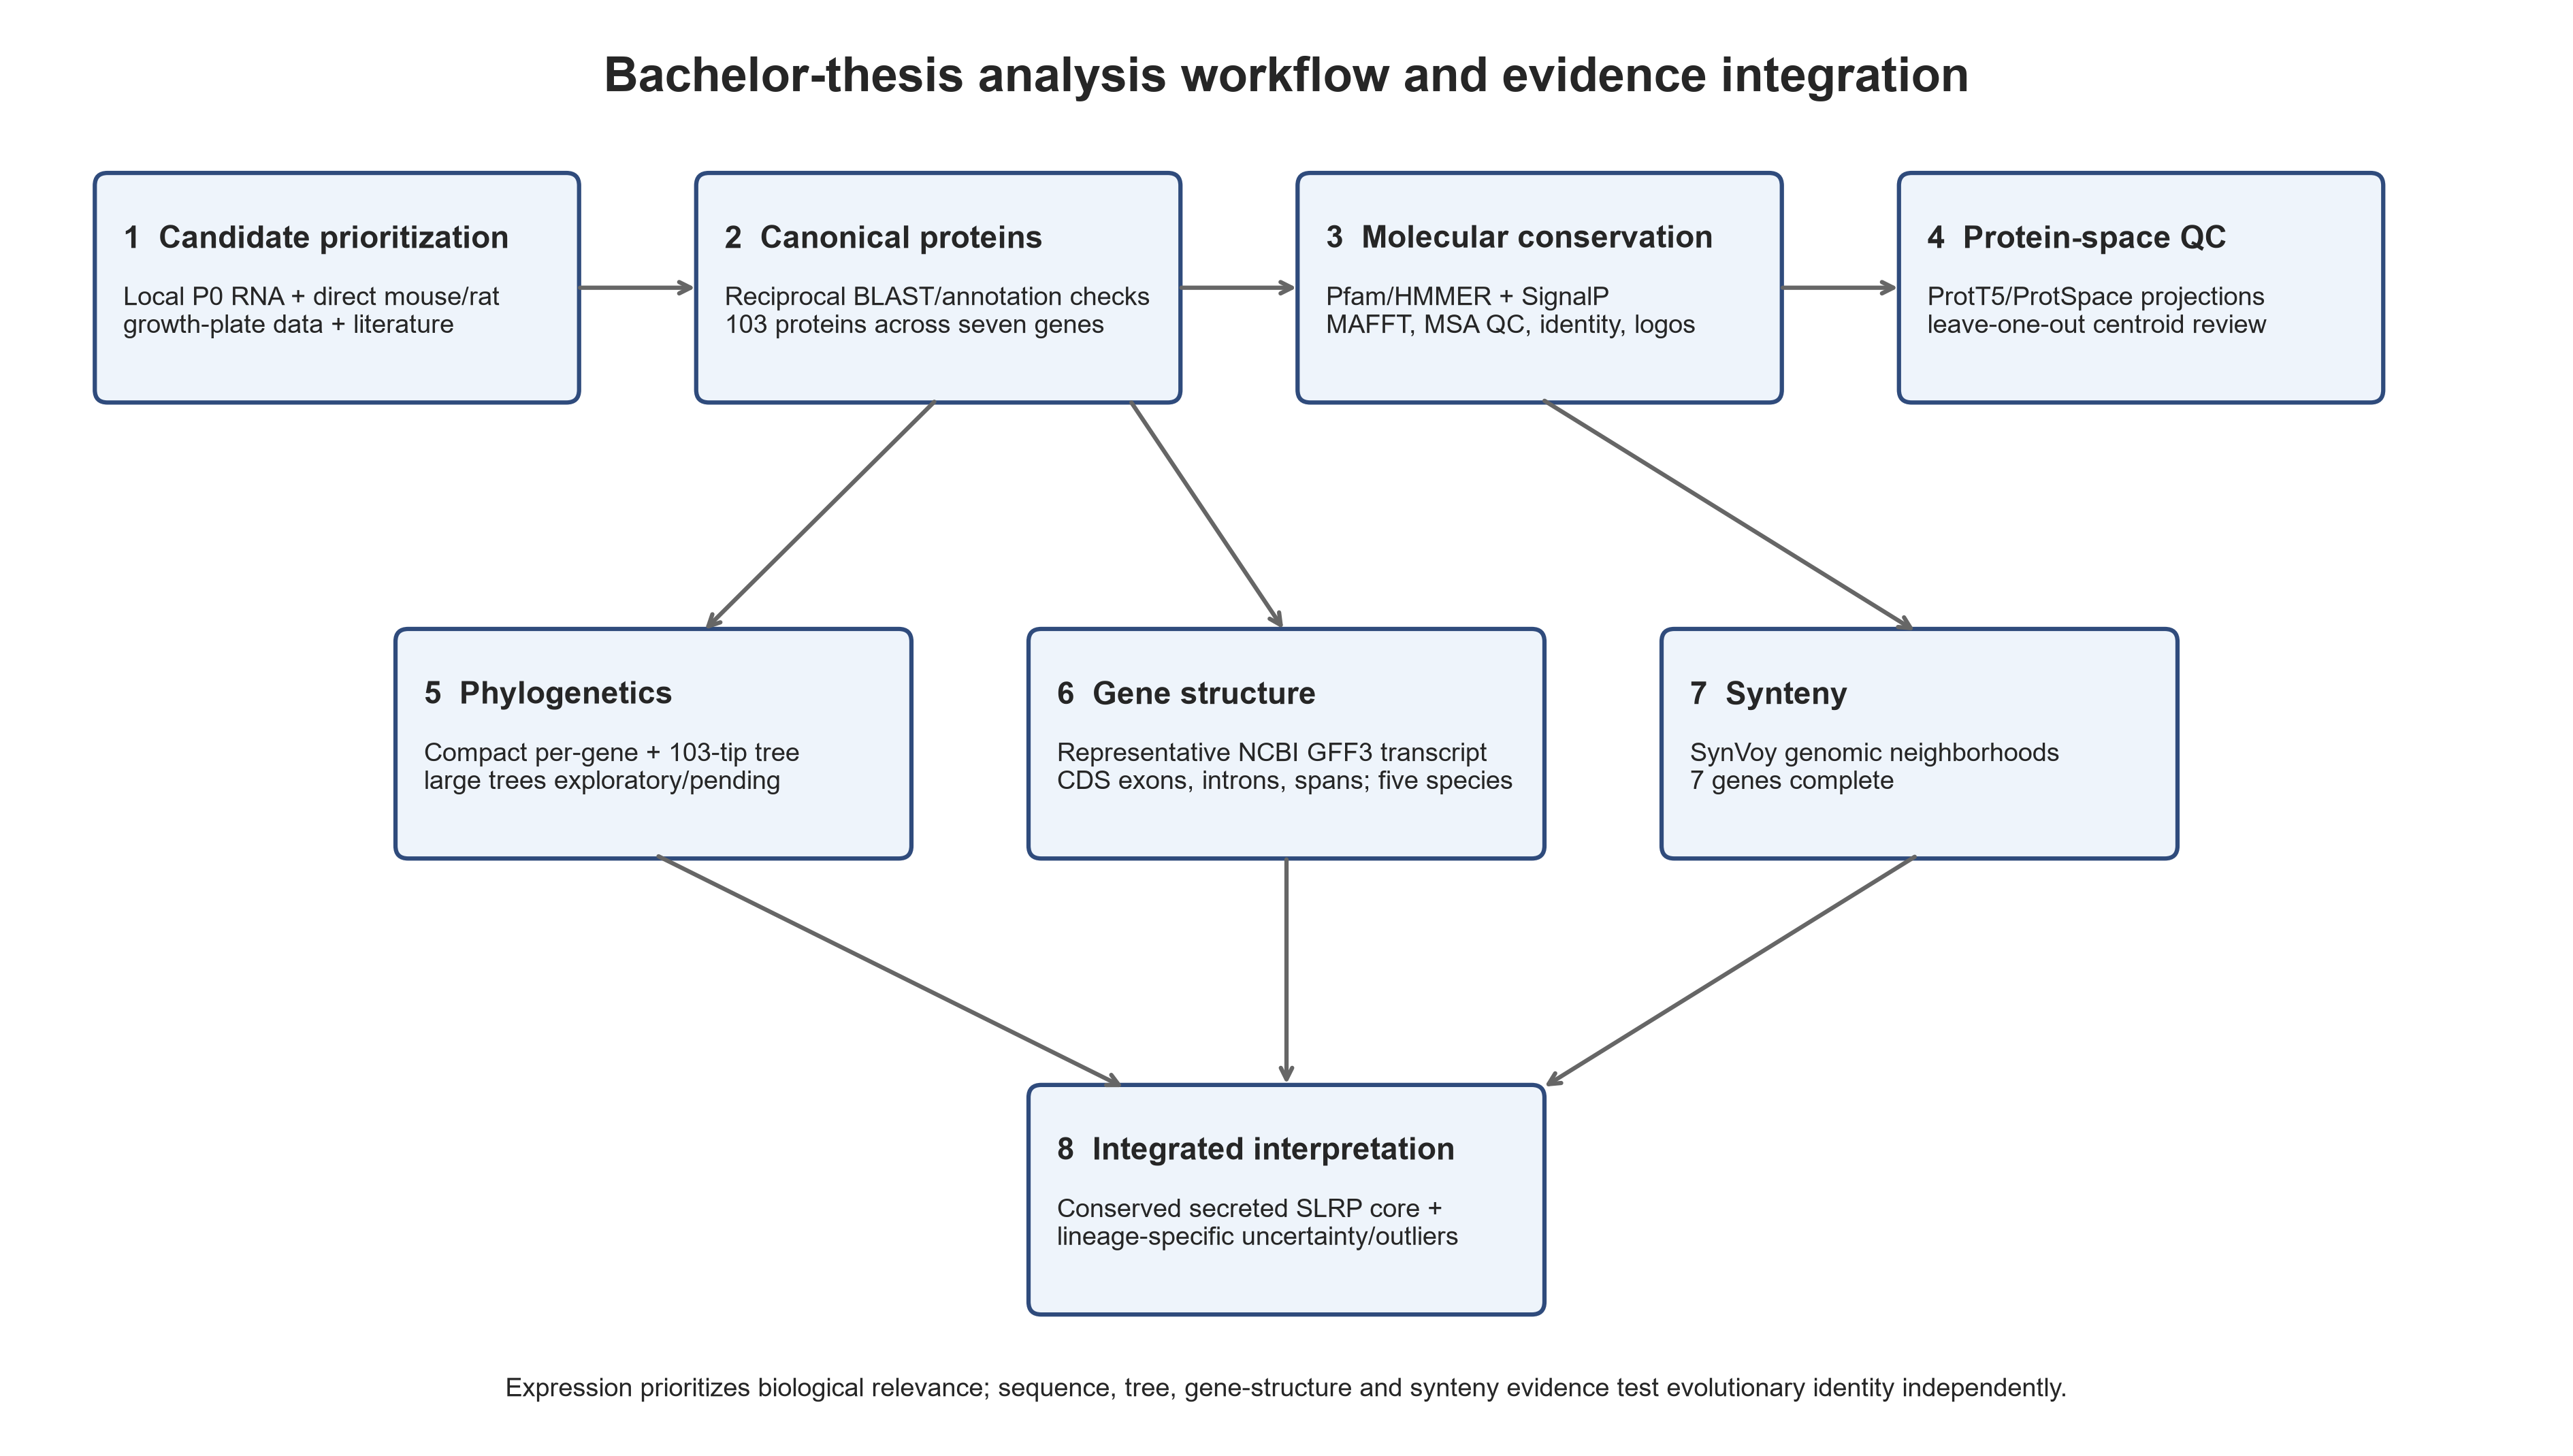
\includegraphics[width=\textwidth,height=0.76\textheight,keepaspectratio]
        {figures/overview/thesis_workflow_overview.png}
    \caption{Overview of the thesis workflow. Expression and literature define
    the biological candidate panel; reciprocal protein searches, domain and
    signal-peptide annotation, alignment, phylogeny, microsynteny, gene
    structure, and manual review provide complementary evidence for ortholog
    plausibility and conservation. Exploratory motif, promoter, embedding, and
    phenotype analyses provide supporting context rather than a single combined
    score.}
    \label{fig:workflow-overview}
\end{figure}

\subsection{Expression datasets and candidate selection}
\label{subsec:rnaseq-expression}

The initial screen used three wild-type samples from the public NCBI Gene
Expression Omnibus study GSE305415 (BioProject PRJNA1305489; raw reads in
NCBI SRA; \url{https://www.ncbi.nlm.nih.gov/geo/query/acc.cgi?acc=GSE305415}).
The selected runs were SRR34978216, SRR34978215, and SRR34978214. The study
obtained Prx1-lineage chondroprogenitors by fluorescence-activated sorting of
digested postnatal-day-0 mouse knee joints \citep{John2026}. The GEO series
description implies RNA extraction after sorting, whereas the individual WT
sample records describe culture toward mature chondrocytes before extraction.
Because this cell-state discrepancy could not be resolved from the deposited
metadata, these samples were treated as P0-derived chondrocyte-lineage material,
not as freshly isolated growth-plate cells. WT1 and WT2 had paired-end runs;
the SRA/ENA run metadata identify WT3 (SRR34978214) as single-end despite the
generic paired-end processing text copied into its GEO sample record.
Previously generated Salmon
\texttt{quant.sf} files stored on the computer were
used because their mapping rates were 81.9--92.0\% and re-extraction reproduced
the previously curated tables. For each sample, transcript TPM values assigned
to the same gene symbol were summed, and the mean, sample standard deviation,
coefficient of variation, and rank of
nine screened SLRPs were calculated across the three wild-type samples. The
original Salmon version and index-building command were not recoverable from the
preserved files; therefore, the analysis is reproducible from the archived
quantifications onward, but this unknown is reported rather than reconstructed.

Four locally available samples from the unrelated ageing atlas PRJNA936435 were
retained only as a descriptive metadata audit. They differed in study, age,
tissue, and replication and were not used for differential expression or for a
growth-plate-versus-other-tissue ratio.

Independent anatomical validation used the processed matrices deposited with
GSE114919. These data contain laser-capture-microdissected proliferative and
hypertrophic zones from mouse and rat growth plates, including tibia at one and
four weeks with five replicates per tibial condition. The authors' normalized
values were retained on their deposited scales. Detection and within-condition
ranks were summarized; values were not pooled with the GSE305415-derived Salmon
TPMs or compared as absolute measurements between species. Bgee 16 expression
calls for mouse, chicken, and zebrafish were used as qualitative context because anatomy,
developmental stage, and assay coverage were not matched among species. Missing
Bgee calls were treated as missing evidence rather than absence of expression.

The final panel was selected from the joint evidence rather than RNA abundance
alone. Selection considered reproducible juvenile expression, direct
growth-plate or cartilage evidence, published skeletal/ECM function, coverage of
SLRP classes I--III, and feasibility of cross-species ortholog analysis. BGN,
DCN, FMOD, PRELP, EPYC, LUM, and OGN were advanced through the full comparative
workflow. DCN also served as the closest paralog control for BGN, and OMD as a
gene-structure and biological-context gene. OGN was designated exploratory
because its growth-plate expression evidence was less consistent. ASPN was kept
as class-I background rather than taken through the full pipeline because its
independent tibial growth-plate support was weaker and less consistent across
the two rodent species, while BGN and DCN already provided the principal
class-I candidate and paralog-control comparison.

\subsection{Reference proteins, ortholog candidates, and manual curation}
\label{subsec:ortholog-search-filtering}

Human proteins served as the query/reference anchors. Candidate proteins were
obtained from NCBI/RefSeq proteomes for a broad chordate panel representing
mammals, bird, reptile, amphibian, teleost and non-teleost bony fish,
cartilaginous fish, jawless vertebrate, and amphioxus comparisons. BLASTP
(version 2.12.0+) was run with an E-value threshold of $10^{-5}$, and reciprocal
searches against the human reference set were used to test gene assignment.
Candidates were screened for compatible annotation, query coverage, protein
length, obvious truncation, and duplicate use of the same accession. A median
length-ratio interval of 0.7--1.3 was used as an automated first-pass filter,
with biologically plausible exceptions assessed manually rather than rejected
solely by length.

The final canonical FASTA contained one nonredundant curated panel per gene.
Manual review in AliView/Jalview emphasized intact N- and C-terminal regions,
conserved cysteine positions, continuous alignment through the LRR-rich region,
absence of large candidate-specific insertions or deletions, and agreement with
reciprocal-hit, phylogenetic, synteny, and SignalP evidence. Exact terminal
identity was not required. Decisions and excluded provenance records were
preserved in the candidate-level confidence table.

\subsection{Domain architecture and signal peptides}
\label{subsec:domain-signalp}

The 103 canonical proteins were scanned with HMMER 3.4 \texttt{hmmscan} against
Pfam-A. Domain hits with independent E-values $\leq 10^{-3}$ were retained, and
LRR/SLRP-family profiles were summarized for each protein. Because related SLRPs
share LRR profiles, this analysis was interpreted as family-membership and
protein-completeness evidence, not gene-specific proof.

Classical secretion signals were predicted with SignalP 6.0 using the eukaryotic
slow-sequential mode. An initial set of 86 retained calls was supplemented by a
final 17-sequence run (job \texttt{6AA7E4B90014723A58E1A86B}), giving predictions
for all 103 canonical proteins (100 positive and three negative). A positive
N-terminal signal is compatible with entry into the
secretory pathway and the expected extracellular localization of SLRPs, but was
not treated as an independent demonstration of in-vivo localization.

\subsection{Multiple-sequence alignment and protein conservation}
\label{subsec:multiple-sequence-alignment}

One alignment per gene was produced with MAFFT 7.505 using
\texttt{--auto}. Pairwise identity was calculated over residue pairs aligned in
both sequences. Per-column occupancy, modal-residue conservation, majority
consensus sequences, species-by-species identity matrices, and sequence logos
were generated from the untrimmed alignments. Untrimmed alignments were retained
for manual biological interpretation so that variable termini and gap-rich
regions remained visible. trimAl 1.5 with \texttt{-automated1} was used to
prepare the combined alignment for phylogenetic analysis.

\subsection{Phylogenetic and embedding analyses}
\label{subsec:phylogenetic-analysis}

Maximum-likelihood phylogenies were inferred with IQ-TREE 2.0.7. ModelFinder
selected the amino-acid substitution model by information criterion
(\texttt{-m MFP}); branch support was estimated with 1,000 SH-aLRT replicates
and 1,000 ultrafast-bootstrap replicates, using automatic thread allocation.
Seven compact per-gene trees were inferred from the canonical MAFFT alignments.
The combined family tree was inferred from the trimAl-filtered 103-protein
alignment. Trees were exported with gene and taxonomic annotation files for
iTOL. Unless an explicit outgroup was applied, trees were interpreted as
unrooted; split support was used for assignment quality and not to infer the
direction or timing of evolution.

As an alignment-independent exploratory check, ProtT5 embeddings were analysed
with ProtSpace projections using PCA, UMAP, and t-SNE. A leave-one-out nearest
gene-centroid test in the original embedding space was used to identify
candidate outliers. Two-dimensional proximity and centroid assignment were
treated as quality-control evidence only.

\subsection{Synteny analysis and manual locus review}
\label{subsec:synteny-analysis}

SynVoy compared the human query locus with 14 non-human target genomes using
the corresponding genome and GFF3 annotation files. Human was therefore the
home-locus anchor rather than an omitted comparison species. The tool's HIGH
and MEDIUM gene-of-interest candidates were parsed after coordinate-ownership
and explicit paralog filtering. Counts refer to retained annotations/candidates,
not a count of proven orthologs. Candidate loci were assigned to P1 detailed,
P2 rapid, or P3 control review according to missing calls, rescue/partial calls,
self-consistency flags, and disagreement with protein or tree evidence.

Runs used protein mode and ten flanking genes. The completed updated-tool BGN
and DCN analyses used MMseqs sensitivity 9.5, non-strict gene-family token
matching, disabled automatic generic presets, an 8-GB MMseqs split-memory
limit, and one iterative-search CPU. For EPYC, FMOD, LUM, OGN, and PRELP, the
current evidence table retained the corresponding completed report and its
run-specific provenance. The completed FMOD refresh was compared with its
historical report and substituted in the final evidence table after the changed
loci were reviewed.

The 98 gene-by-target combinations underwent an exact-assembly locus audit:
the canonical protein accession was searched in the GFF3 used by SynVoy and,
where present, compared with the best post-ownership candidate coordinate.
The 68 P2 rows and four P3 controls were screened primarily by this
reproducible accession--locus comparison; conflicts and missing accessions
were escalated. The 26 P1 exceptions received detailed feature and
neighbourhood review. For these rows, the
annotated symbol or uncharacterized model, strand, accession, and informative
non-SLRP flanking genes were recorded, and gene order was compared after
orienting both blocks relative to the focal gene. Fifteen genes on each side
were used by default; the annotation-rich but \texttt{LOC}-dominated catshark BGN
region was broadened to 40 genes per side. Locus evidence was integrated with
reciprocal protein, domain, SignalP, embedding-QC, and tree results.
Selected difficult loci were also inspected visually in NCBI Genome Data Viewer
against the exact target assembly and SynVoy neighbourhood plot. The 98-row
audit should not be interpreted as 98 independent visual GDV confirmations.

For the unusually long elephant-shark FMOD-like model
(\texttt{XP\_007897806.2}), all nine CDS features were reconstructed from the
exact SynVoy FASTA/GFF3 pair and translated in transcript order. Translation
completeness, terminal and internal stops, and GFF3 phase values were recorded.
The protein was compared by local BLASTP with human BGN, DCN, ASPN, FMOD,
PRELP, LUM, EPYC, and OGN references, and independently scanned against the
local Pfam-A database with HMMER 3.4. Hydrophobic segments were inspected
directly but were not reported as formal SignalP predictions.

FASTA and GFF3 sequence identifiers were audited before interpretation. The
opossum pair used by the completed reports failed this check because six
chromosome accessions differed by version and three GFF3 scaffolds were absent
from the FASTA. All opossum calls in the frozen evidence table were therefore
classified as not assessable. A replacement GCF\_027887165.2 pair was later
validated (13/13 annotated sequence identifiers matched exactly), but the
gene-level reruns were not complete when the table was frozen. Independently
supported opossum proteins remained eligible for protein, alignment, and tree
analyses. Missing annotations were otherwise
described as annotation-limited unless GFF3 and protein-to-genome evidence
independently supported gene loss. SynVoy was thus used as qualitative locus-
level orthology support, not as a binary test.

For a descriptive species-lineage comparison, canonical proteins were grouped
by sampled species and their median forward amino-acid identity to the human
query was calculated. The numbers of supported, watch-list, and
needs-inspection protein models and the accepted, tentative, ambiguous, and
rejected synteny
decisions were summarized per species. These summaries were not treated as an
evolutionary clock: species with different numbers of retained genes were not
compared inferentially, and missing candidates were not interpreted as gene
loss.

\subsection{Full representative transcript and coding-gene structure}
\label{subsec:gene-structure}

Gene, transcript, exon, and CDS relationships were parsed from the same NCBI
GFF3 annotations used for human, mouse, cow, chicken, and zebrafish genome
analyses. One representative protein-coding transcript was selected for each of
BGN, DCN, FMOD, PRELP, EPYC, LUM, OGN, and OMD in each species. Transcript strand,
full exon structure, CDS blocks, exon-derived 5-prime and 3-prime UTR segments,
summed CDS length, translated protein length, and genomic span were recorded.
Negative-strand models were displayed in transcript orientation. CDS sequences
were reconstructed directly from indexed genome assemblies and translated to
test divisibility by three, start methionine, terminal stop codon, and internal
stop codons. GFF3 phase values were checked against cumulative CDS length.

Coding boundaries were projected onto protein coordinates. For every junction
present in all five representatives, intron phase and the range of amino-acid
boundary positions were compared across species. All annotated protein-coding
transcripts at each selected locus were also inventoried to determine whether
transcript choice could change CDS-exon count or protein length. Predicted
\texttt{XM\_} models were audited separately. This is a representative-model
comparison with an annotation-level isoform-sensitivity check; it does not show
which alternative isoform is expressed in the growth plate. UTR differences
were treated as annotation-sensitive descriptive observations.

The 40 reconstructed representative translations were rescanned against the
local Pfam-A database with HMMER 3.4. Significant domain hits
($i$-value $\leq10^{-3}$) were projected onto cumulative coding-exon
coordinates. This tested whether conserved SLRP/LRR architecture spans the same
coding framework, but domain--exon overlap was not interpreted as evidence that
individual exons encode independent biochemical modules.

Representative structure translations were cross-referenced against the final
canonical protein panel by gene, species, accession, and global amino-acid
alignment. This audit distinguished exact or alternative accessions from
different teleost co-orthologs and from records excluded during protein
curation. Passing transcript and CDS quality control was therefore treated as
evidence for a technically coherent annotation, not by itself as validation of
gene-specific orthology.

\subsection{Supplementary coding-sequence constraint}
\label{subsec:codon-constraint}

For each gene, the five reconstructed representative proteins were aligned with
MAFFT and their CDSs were back-translated through the protein alignment.
Gap-containing and invalid codon pairs were omitted. Human was compared
separately with mouse, cow, chicken, and zebrafish using the pairwise
Nei--Gojobori method implemented in Biopython \citep{NeiGojobori1986}. The known
ASPN-like chicken BGN-locus product was excluded because it is not a secure BGN
ortholog. Ratios with undefined or non-positive $d_S$ were reported as
unavailable, and comparisons with $d_S\geq2$ were flagged for possible
synonymous-site saturation. These whole-sequence pairwise estimates are a
descriptive constraint check, not a branch-, site-, or branch-site selection
test.

\subsection{Supplementary mature-protein motif analysis}
\label{subsec:protein-motifs}

SignalP-positive signal peptides were removed at the predicted cleavage site to
focus motif analysis on mature-protein proxies. The three SignalP-negative
proteins (whale-shark BGN, opossum DCN, and spotted-gar OGN) remained
untrimmed. The motif input was regenerated after all 103 final SignalP calls
were available. MEME 5.5.8 was run in protein ZOOPS mode with motif
widths of 6--40 amino acids and an E-value stopping threshold of 0.05
\citep{Bailey2015MEME}. Each gene-specific MEME model was scanned against all 103
proteins with MAST. The sum of $-\log_{10}(p)$ over significant MAST motif hits
was used only as a visualization/ranking score. STREME compared each gene's
proteins against the other six genes with no holdout set
\citep{Bailey2021STREME}. These analyses test recurrent sequence patterns and
candidate outliers; they do not assign biochemical function to motifs.

\subsection{Exploratory comparative promoter analysis}
\label{subsec:promoter-analysis}

Promoters were extracted for the same representative transcripts and NCBI
assemblies used in the five-species gene-structure analysis. Strand-aware core
($-500$ to $+100$ bp) and proximal ($-2{,}000$ to $+200$ bp) windows were defined
relative to the annotated transcription start site and extracted with samtools
1.24. Sequence length, clipping, ambiguous bases, and GC content were checked.

STREME 5.5.8 was run on proximal promoters with motif widths 6--15 bp,
dinucleotide-shuffled controls, and random seed 20260826. The global search used
all 35 promoters; each gene-level search used five promoters as positives and
the remaining 30 as controls. Tomtom compared de-novo motifs with the 1,019
nonredundant vertebrate CORE motifs in JASPAR 2026
\citep{Ovek2026JASPAR}. AME used Fisher's exact test with total-hit scoring and
dinucleotide-shuffled controls for both the full database and a 40-profile panel
of cartilage, hypoxia, osteogenesis, and signalling-related transcription
factors. FIMO scans used a strict q-value threshold of 0.05; a separate
$p\leq10^{-4}$ scan was retained only as uncorrected exploratory recurrence.
Motif occurrences were not described as transcription-factor binding sites.

\subsection{Curated phenotype associations}
\label{subsec:phenotype-analysis}

Mouse phenotype associations were downloaded from Mouse Genome Informatics on
26 August 2026 using \texttt{MGI\_GenePheno.rpt} and
\texttt{MGI\_PhenoGenoMP.rpt}; Mammalian Phenotype ontology release 22 July 2026
was used to propagate broad skeletal, cartilage, joint, growth, and ECM-related
categories \citep{Baldarelli2024MGI}. Single-gene and compound genotypes were
distinguished. Human annotations used the pinned Human Phenotype Ontology
release v2026-06-23, including \texttt{genes\_to\_phenotype.txt} and
\texttt{genes\_to\_disease.txt} \citep{Gargano2024HPO}. Source checksums were
stored with the analysis. Counts were interpreted as annotation depth, not
effect size, and lack of a database record was treated as absence of curated
evidence rather than absence of biological function.


% ------------------------------------------------------------
% References
% ------------------------------------------------------------
\newpage
\RaggedRight
\bibliographystyle{plainnat}
\bibliography{bibliography}

% ------------------------------------------------------------
% Supplementary material
% ------------------------------------------------------------
\newpage
\appendix
\section{Supplementary Material}
\label{sec:supplementary}
\subsection{Electronic supplementary tables}

The electronic result package contains the following thesis-facing tables:

\begin{itemize}
    \item the final gene-level evidence table for the seven comparative genes
    and OMD context;
    \item the 107-row candidate-level confidence and provenance table;
    \item the 103-row integrated protein/domain/MSA/SignalP table and per-gene
    conservation summaries;
    \item representative gene-structure and SynVoy gene-by-species evidence
    tables;
    \item mature-protein MEME/STREME/MAST summaries;
    \item promoter-sequence QC, corrected enrichment, and exploratory recurrence
    tables; and
    \item MGI/MP and HPO phenotype evidence summaries.
\end{itemize}

Accession, species, manual-decision, and source-provenance fields are retained so
that excluded or tentative candidates remain auditable rather than disappearing
from the final package.

\subsection{Electronic supplementary figures}

Supplementary figures include the seven gene-specific phylogenies and sequence
logos, a replicate-level GSE114919 expression display, eight representative
CDS-structure plots, ProtSpace projections, SynVoy
confidence/review summaries, the mature-protein motif-model matrix, promoter GC
and motif summaries, and the curated mouse phenotype heatmap. Individual
SignalP plots and tool-native motif reports are retained as diagnostics rather
than interpreted as independent biological results.

The original ZIP contained seven separate CDS-structure plots (BGN, EPYC, FMOD,
LUM, OGN, OMD, and PRELP). DCN was added later and is represented in the updated
eight-gene overview and full-transcript figures rather than by an obsolete or
newly invented per-gene panel.

\newcommand{\thesissuppfigure}[3]{%
\begin{figure}[p]
    \centering
    \includegraphics[width=\textwidth,height=0.80\textheight,keepaspectratio]{#1}
    \caption{#2}
    \label{#3}
\end{figure}%
}

\clearpage
\subsubsection{Expression context}

\thesissuppfigure
{figures/expression/expression_age_and_bgee_overview.png}
{Age-, zone-, species-, and Bgee-based expression context for the seven-gene
panel. The comparisons are descriptive and retain their dataset-specific
scales; missing Bgee calls are interpreted as missing database evidence rather
than absence of expression.}
{fig:supp-expression-context}

\thesissuppfigure
{figures/expression/gse114919_slrp_replicates.png}
{Replicate-level expression of the nine screened SLRPs in the deposited
GSE114919 mouse and rat growth-plate matrices. Points are biological replicates
and black bars are condition means on the authors' published normalized-value
scale. Conditions encode species, age, bone, and proliferative or hypertrophic
zone. Absolute values are not compared between species and no inferential test
is implied.}
{fig:supp-gse114919-replicates}

\clearpage
\subsubsection{Phylogenetic detail}

\thesissuppfigure
{figures/phylogeny/compact_per_gene_trees.png}
{Maximum-likelihood phylogenies of the seven curated gene-specific protein
sets. Models were selected independently and branch support was estimated with
1,000 SH-aLRT and 1,000 ultrafast-bootstrap replicates. All trees are unrooted;
their display orientation does not represent evolutionary direction.}
{fig:supp-per-gene-trees}

\thesissuppfigure
{figures/phylogeny/phylogenetic_result_overview.png}
{Phylogenetic result and provenance overview. The curated compact trees are the
source of thesis conclusions. Legacy very-large tree products are shown only as
an analysis audit because their former header parser could collapse unrelated
loci with repeated isoform labels; corrected locus-filtered inputs exist, but
their long-tree inference remains optional.}
{fig:supp-phylogeny-audit}

\clearpage
\subsubsection{Sequence-conservation logos}

\thesissuppfigure
{figures/protein/sequence_logos/BGN_sequence_logo.png}
{Occupancy-weighted amino-acid sequence logo for the curated BGN alignment.
Coordinates are alignment columns rather than human-protein residue numbers.}
{fig:supp-logo-bgn}

\thesissuppfigure
{figures/protein/sequence_logos/DCN_sequence_logo.png}
{Occupancy-weighted amino-acid sequence logo for the curated DCN alignment.
Coordinates are alignment columns rather than human-protein residue numbers.}
{fig:supp-logo-dcn}

\thesissuppfigure
{figures/protein/sequence_logos/EPYC_sequence_logo.png}
{Occupancy-weighted amino-acid sequence logo for the curated EPYC alignment.
Coordinates are alignment columns rather than human-protein residue numbers.}
{fig:supp-logo-epyc}

\thesissuppfigure
{figures/protein/sequence_logos/FMOD_sequence_logo.png}
{Occupancy-weighted amino-acid sequence logo for the curated FMOD alignment.
Coordinates are alignment columns rather than human-protein residue numbers.}
{fig:supp-logo-fmod}

\thesissuppfigure
{figures/protein/sequence_logos/LUM_sequence_logo.png}
{Occupancy-weighted amino-acid sequence logo for the curated LUM alignment.
Coordinates are alignment columns rather than human-protein residue numbers.}
{fig:supp-logo-lum}

\thesissuppfigure
{figures/protein/sequence_logos/OGN_sequence_logo.png}
{Occupancy-weighted amino-acid sequence logo for the curated OGN alignment.
The continuous conserved core is retained despite greater overall divergence.}
{fig:supp-logo-ogn}

\thesissuppfigure
{figures/protein/sequence_logos/PRELP_sequence_logo.png}
{Occupancy-weighted amino-acid sequence logo for the curated PRELP alignment.
Coordinates are alignment columns rather than human-protein residue numbers.}
{fig:supp-logo-prelp}

\clearpage
\subsubsection{Gene-structure detail}

\thesissuppfigure
{figures/gene_structure/full_gene_structure_5species.png}
{Full representative transcript organization for seven comparative genes and
OMD in human, mouse, cow, chicken, and zebrafish. Grey shows complete exon
extent, blue and orange denote derived UTR segments, and gene-specific colours
denote CDS. Coding structure is more stable than intron spacing and annotated
UTR length.}
{fig:supp-full-gene-structure}

\thesissuppfigure
{figures/gene_structure/coding_exon_splice_phase_map.png}
{Coding-exon boundaries and intron phases across five vertebrates. All 26
homologous coding junctions retain intron phase even where exact boundary
positions shift modestly.}
{fig:supp-splice-phase}

\thesissuppfigure
{figures/gene_structure/human_domain_exon_architecture.png}
{Human LRR-family Pfam hits projected onto coding exons. Domain-model overlap
with multiple exons links the protein architecture to the conserved coding
framework but does not imply that each exon is an independent functional
module.}
{fig:supp-domain-exon}

\thesissuppfigure
{figures/gene_structure/per_gene/BGN_cds_gene_structure_5species.png}
{Representative BGN CDS organization in five vertebrates. Boxes are CDS
segments and connecting lines are intervening genomic sequence in transcript
orientation.}
{fig:supp-structure-bgn}

\thesissuppfigure
{figures/gene_structure/per_gene/EPYC_cds_gene_structure_5species.png}
{Representative EPYC CDS organization in five vertebrates. Differences in
total span mainly reflect intervening sequence and transcript choice.}
{fig:supp-structure-epyc}

\thesissuppfigure
{figures/gene_structure/per_gene/FMOD_cds_gene_structure_5species.png}
{Representative FMOD CDS organization in five vertebrates.}
{fig:supp-structure-fmod}

\thesissuppfigure
{figures/gene_structure/per_gene/LUM_cds_gene_structure_5species.png}
{Representative LUM CDS organization in five vertebrates.}
{fig:supp-structure-lum}

\thesissuppfigure
{figures/gene_structure/per_gene/OGN_cds_gene_structure_5species.png}
{Representative OGN CDS organization in five vertebrates.}
{fig:supp-structure-ogn}

\thesissuppfigure
{figures/gene_structure/per_gene/OMD_cds_gene_structure_5species.png}
{Representative OMD CDS organization in five vertebrates. OMD is a context gene
and was not advanced through the complete seven-gene comparative workflow.}
{fig:supp-structure-omd}

\thesissuppfigure
{figures/gene_structure/per_gene/PRELP_cds_gene_structure_5species.png}
{Representative PRELP CDS organization in five vertebrates.}
{fig:supp-structure-prelp}

\clearpage
\subsubsection{Coding constraint and protein-space analyses}

\thesissuppfigure
{figures/evolutionary_rates/pairwise_dn_ds_human_reference.png}
{Human-reference pairwise coding-sequence constraint for seven comparative
genes and OMD. All 25 finite NG86 estimates are below one. Undefined or non-
positive synonymous distances are not plotted, and high-$d_S$ comparisons are
interpreted with saturation caution.}
{fig:supp-dnds}

\thesissuppfigure
{figures/protspace/protspace_canonical_projections.png}
{PCA, UMAP, and t-SNE projections of ProtT5 embeddings for the canonical
proteins and controls. These projections provide exploratory quality control;
visual proximity does not establish orthology or biological function.}
{fig:supp-protspace}

\clearpage
\subsubsection{Protein motifs}

\thesissuppfigure
{figures/motifs/protein_gene_motif_model_matrix.png}
{Compatibility of the 103 canonical proteins with the seven gene-specific
mature-protein MEME models. Every protein scores most strongly against its own
gene model, but the models were learned and evaluated on the same curated panel
and are not an independent accuracy estimate.}
{fig:supp-motif-matrix}

\thesissuppfigure
{figures/motifs/protein_candidate_motif_model_margins.png}
{Per-candidate margin between the assigned-gene motif model and the strongest
alternative model. Margins are supporting sequence-classification evidence and
must not be interpreted as validated functional binding motifs.}
{fig:supp-motif-margins}

\clearpage
\subsubsection{Promoter analysis}

\thesissuppfigure
{figures/regulatory/promoter_proximal_gc_heatmap.png}
{GC composition of strand-aware $-2{,}000/+200$-bp proximal promoters from 35
representative gene--species loci. All windows passed sequence-length and
ambiguity checks.}
{fig:supp-promoter-gc}

\thesissuppfigure
{figures/regulatory/promoter_targeted_tf_ame_enrichment.png}
{AME results for the targeted cartilage/osteogenesis transcription-factor
motif panel. HIF1A has the strongest raw result, but no targeted motif passes
the panel-corrected threshold; the figure does not demonstrate shared
regulation.}
{fig:supp-promoter-ame}

\thesissuppfigure
{figures/regulatory/promoter_targeted_tf_species_recurrence.png}
{Exploratory recurrence of targeted motif matches across five species at an
uncorrected FIMO threshold. The strict $q\leq0.05$ scan returned no sites, so
these patterns are hypotheses rather than conserved binding sites.}
{fig:supp-promoter-recurrence}

\clearpage
\subsubsection{Phenotype evidence}

\thesissuppfigure
{figures/phenotypes/mgi_single_gene_phenotype_heatmap.png}
{Breadth of curated single-gene mouse phenotype annotations for the seven
SLRPs. Counts represent database annotation coverage, not phenotype severity,
effect size, or cross-gene biological importance.}
{fig:supp-mgi-phenotypes}

\subsection{Manual-review records}

The manual sequence record documents the retained opossum and zebrafish OGN
proteins, tentative spotted-gar OGN and whale-shark EPYC proteins, and excluded
amphioxus SLRP-like candidate. The synteny review table uses the controlled
vocabulary \emph{accepted}, \emph{tentative}, \emph{rejected}, and
\emph{ambiguous}. All 98 rows have exact-assembly GFF/accession-based
decisions; the 25 prioritized exceptions received more detailed feature and
flanking-gene review. Only selected disputed cases were cross-checked visually
in NCBI Genome Data Viewer. The decisions integrate the target gene model,
informative flanking genes, reciprocal protein evidence, and tree placement.


\end{document}
